% Options for packages loaded elsewhere
\PassOptionsToPackage{unicode}{hyperref}
\PassOptionsToPackage{hyphens}{url}
%
\documentclass[
]{article}
\usepackage{amsmath,amssymb}
\usepackage{iftex}
\ifPDFTeX
  \usepackage[T1]{fontenc}
  \usepackage[utf8]{inputenc}
  \usepackage{textcomp} % provide euro and other symbols
\else % if luatex or xetex
  \usepackage{unicode-math} % this also loads fontspec
  \defaultfontfeatures{Scale=MatchLowercase}
  \defaultfontfeatures[\rmfamily]{Ligatures=TeX,Scale=1}
\fi
\usepackage{lmodern}
\ifPDFTeX\else
  % xetex/luatex font selection
\fi
% Use upquote if available, for straight quotes in verbatim environments
\IfFileExists{upquote.sty}{\usepackage{upquote}}{}
\IfFileExists{microtype.sty}{% use microtype if available
  \usepackage[]{microtype}
  \UseMicrotypeSet[protrusion]{basicmath} % disable protrusion for tt fonts
}{}
\makeatletter
\@ifundefined{KOMAClassName}{% if non-KOMA class
  \IfFileExists{parskip.sty}{%
    \usepackage{parskip}
  }{% else
    \setlength{\parindent}{0pt}
    \setlength{\parskip}{6pt plus 2pt minus 1pt}}
}{% if KOMA class
  \KOMAoptions{parskip=half}}
\makeatother
\usepackage{xcolor}
\usepackage[margin=1in]{geometry}
\usepackage{color}
\usepackage{fancyvrb}
\newcommand{\VerbBar}{|}
\newcommand{\VERB}{\Verb[commandchars=\\\{\}]}
\DefineVerbatimEnvironment{Highlighting}{Verbatim}{commandchars=\\\{\}}
% Add ',fontsize=\small' for more characters per line
\usepackage{framed}
\definecolor{shadecolor}{RGB}{248,248,248}
\newenvironment{Shaded}{\begin{snugshade}}{\end{snugshade}}
\newcommand{\AlertTok}[1]{\textcolor[rgb]{0.94,0.16,0.16}{#1}}
\newcommand{\AnnotationTok}[1]{\textcolor[rgb]{0.56,0.35,0.01}{\textbf{\textit{#1}}}}
\newcommand{\AttributeTok}[1]{\textcolor[rgb]{0.13,0.29,0.53}{#1}}
\newcommand{\BaseNTok}[1]{\textcolor[rgb]{0.00,0.00,0.81}{#1}}
\newcommand{\BuiltInTok}[1]{#1}
\newcommand{\CharTok}[1]{\textcolor[rgb]{0.31,0.60,0.02}{#1}}
\newcommand{\CommentTok}[1]{\textcolor[rgb]{0.56,0.35,0.01}{\textit{#1}}}
\newcommand{\CommentVarTok}[1]{\textcolor[rgb]{0.56,0.35,0.01}{\textbf{\textit{#1}}}}
\newcommand{\ConstantTok}[1]{\textcolor[rgb]{0.56,0.35,0.01}{#1}}
\newcommand{\ControlFlowTok}[1]{\textcolor[rgb]{0.13,0.29,0.53}{\textbf{#1}}}
\newcommand{\DataTypeTok}[1]{\textcolor[rgb]{0.13,0.29,0.53}{#1}}
\newcommand{\DecValTok}[1]{\textcolor[rgb]{0.00,0.00,0.81}{#1}}
\newcommand{\DocumentationTok}[1]{\textcolor[rgb]{0.56,0.35,0.01}{\textbf{\textit{#1}}}}
\newcommand{\ErrorTok}[1]{\textcolor[rgb]{0.64,0.00,0.00}{\textbf{#1}}}
\newcommand{\ExtensionTok}[1]{#1}
\newcommand{\FloatTok}[1]{\textcolor[rgb]{0.00,0.00,0.81}{#1}}
\newcommand{\FunctionTok}[1]{\textcolor[rgb]{0.13,0.29,0.53}{\textbf{#1}}}
\newcommand{\ImportTok}[1]{#1}
\newcommand{\InformationTok}[1]{\textcolor[rgb]{0.56,0.35,0.01}{\textbf{\textit{#1}}}}
\newcommand{\KeywordTok}[1]{\textcolor[rgb]{0.13,0.29,0.53}{\textbf{#1}}}
\newcommand{\NormalTok}[1]{#1}
\newcommand{\OperatorTok}[1]{\textcolor[rgb]{0.81,0.36,0.00}{\textbf{#1}}}
\newcommand{\OtherTok}[1]{\textcolor[rgb]{0.56,0.35,0.01}{#1}}
\newcommand{\PreprocessorTok}[1]{\textcolor[rgb]{0.56,0.35,0.01}{\textit{#1}}}
\newcommand{\RegionMarkerTok}[1]{#1}
\newcommand{\SpecialCharTok}[1]{\textcolor[rgb]{0.81,0.36,0.00}{\textbf{#1}}}
\newcommand{\SpecialStringTok}[1]{\textcolor[rgb]{0.31,0.60,0.02}{#1}}
\newcommand{\StringTok}[1]{\textcolor[rgb]{0.31,0.60,0.02}{#1}}
\newcommand{\VariableTok}[1]{\textcolor[rgb]{0.00,0.00,0.00}{#1}}
\newcommand{\VerbatimStringTok}[1]{\textcolor[rgb]{0.31,0.60,0.02}{#1}}
\newcommand{\WarningTok}[1]{\textcolor[rgb]{0.56,0.35,0.01}{\textbf{\textit{#1}}}}
\usepackage{longtable,booktabs,array}
\usepackage{calc} % for calculating minipage widths
% Correct order of tables after \paragraph or \subparagraph
\usepackage{etoolbox}
\makeatletter
\patchcmd\longtable{\par}{\if@noskipsec\mbox{}\fi\par}{}{}
\makeatother
% Allow footnotes in longtable head/foot
\IfFileExists{footnotehyper.sty}{\usepackage{footnotehyper}}{\usepackage{footnote}}
\makesavenoteenv{longtable}
\usepackage{graphicx}
\makeatletter
\def\maxwidth{\ifdim\Gin@nat@width>\linewidth\linewidth\else\Gin@nat@width\fi}
\def\maxheight{\ifdim\Gin@nat@height>\textheight\textheight\else\Gin@nat@height\fi}
\makeatother
% Scale images if necessary, so that they will not overflow the page
% margins by default, and it is still possible to overwrite the defaults
% using explicit options in \includegraphics[width, height, ...]{}
\setkeys{Gin}{width=\maxwidth,height=\maxheight,keepaspectratio}
% Set default figure placement to htbp
\makeatletter
\def\fps@figure{htbp}
\makeatother
\setlength{\emergencystretch}{3em} % prevent overfull lines
\providecommand{\tightlist}{%
  \setlength{\itemsep}{0pt}\setlength{\parskip}{0pt}}
\setcounter{secnumdepth}{5}
% definitions for citeproc citations
\NewDocumentCommand\citeproctext{}{}
\NewDocumentCommand\citeproc{mm}{%
  \begingroup\def\citeproctext{#2}\cite{#1}\endgroup}
\makeatletter
 % allow citations to break across lines
 \let\@cite@ofmt\@firstofone
 % avoid brackets around text for \cite:
 \def\@biblabel#1{}
 \def\@cite#1#2{{#1\if@tempswa , #2\fi}}
\makeatother
\newlength{\cslhangindent}
\setlength{\cslhangindent}{1.5em}
\newlength{\csllabelwidth}
\setlength{\csllabelwidth}{3em}
\newenvironment{CSLReferences}[2] % #1 hanging-indent, #2 entry-spacing
 {\begin{list}{}{%
  \setlength{\itemindent}{0pt}
  \setlength{\leftmargin}{0pt}
  \setlength{\parsep}{0pt}
  % turn on hanging indent if param 1 is 1
  \ifodd #1
   \setlength{\leftmargin}{\cslhangindent}
   \setlength{\itemindent}{-1\cslhangindent}
  \fi
  % set entry spacing
  \setlength{\itemsep}{#2\baselineskip}}}
 {\end{list}}
\usepackage{calc}
\newcommand{\CSLBlock}[1]{\hfill\break\parbox[t]{\linewidth}{\strut\ignorespaces#1\strut}}
\newcommand{\CSLLeftMargin}[1]{\parbox[t]{\csllabelwidth}{\strut#1\strut}}
\newcommand{\CSLRightInline}[1]{\parbox[t]{\linewidth - \csllabelwidth}{\strut#1\strut}}
\newcommand{\CSLIndent}[1]{\hspace{\cslhangindent}#1}
\usepackage{graphicx}
\usepackage{titling}

\pretitle{}
\posttitle{}

\preauthor{}
\postauthor{}

\predate{}
\postdate{}

\renewcommand{\maketitle}{
  \begin{center}
    \vspace*{2cm}
    {\Huge \textbf{Part A, Topic 1 - COVID-19}}\\[1.5cm]  % Title
    
\includegraphics[width=0.3\textwidth]{Monash University.png}\\[1.5cm]  % Logo (logo.png must be in the same folder)
    {\LARGE \textbf{Lance Belen}}\\[1.5cm]  % Author
    \vspace*{1cm}
    \today
    \vfill
  \end{center}
  \newpage
}
\ifLuaTeX
  \usepackage{selnolig}  % disable illegal ligatures
\fi
\usepackage{bookmark}
\IfFileExists{xurl.sty}{\usepackage{xurl}}{} % add URL line breaks if available
\urlstyle{same}
\hypersetup{
  pdftitle={Part A, Topic 1 - COVID-19},
  pdfauthor={Lance Belen},
  hidelinks,
  pdfcreator={LaTeX via pandoc}}

\title{Part A, Topic 1 - COVID-19}
\author{Lance Belen}
\date{2 June 2025}

\begin{document}
\maketitle

{
\setcounter{tocdepth}{2}
\tableofcontents
}
\newpage

\section{Data Wrangling and
Integration}\label{data-wrangling-and-integration}

First, load the packages needed.

\begin{Shaded}
\begin{Highlighting}[]
\FunctionTok{options}\NormalTok{(}\AttributeTok{repos =} \FunctionTok{c}\NormalTok{(}\AttributeTok{CRAN =} \StringTok{"https://cloud.r{-}project.org/"}\NormalTok{))}

\ControlFlowTok{if}\NormalTok{ (}\SpecialCharTok{!}\FunctionTok{requireNamespace}\NormalTok{(}\StringTok{"tidyverse"}\NormalTok{, }\AttributeTok{quietly =} \ConstantTok{TRUE}\NormalTok{)) \{}
  \FunctionTok{install.packages}\NormalTok{(}\StringTok{"tidyverse"}\NormalTok{)}
\NormalTok{\}}
\ControlFlowTok{if}\NormalTok{ (}\SpecialCharTok{!}\FunctionTok{requireNamespace}\NormalTok{(}\StringTok{"lubridate"}\NormalTok{, }\AttributeTok{quietly =} \ConstantTok{TRUE}\NormalTok{)) \{}
  \FunctionTok{install.packages}\NormalTok{(}\StringTok{"lubridate"}\NormalTok{)}
\NormalTok{\}}
\ControlFlowTok{if}\NormalTok{ (}\SpecialCharTok{!}\FunctionTok{requireNamespace}\NormalTok{(}\StringTok{"impute"}\NormalTok{, }\AttributeTok{quietly =} \ConstantTok{TRUE}\NormalTok{)) \{}
  \FunctionTok{install.packages}\NormalTok{(}\StringTok{"impute"}\NormalTok{)}
\NormalTok{\}}
\ControlFlowTok{if}\NormalTok{ (}\SpecialCharTok{!}\FunctionTok{requireNamespace}\NormalTok{(}\StringTok{"dplyr"}\NormalTok{, }\AttributeTok{quietly =} \ConstantTok{TRUE}\NormalTok{)) \{}
  \FunctionTok{install.packages}\NormalTok{(}\StringTok{"dplyr"}\NormalTok{)}
\NormalTok{\}}
\ControlFlowTok{if}\NormalTok{ (}\SpecialCharTok{!}\FunctionTok{requireNamespace}\NormalTok{(}\StringTok{"magrittr"}\NormalTok{, }\AttributeTok{quietly =} \ConstantTok{TRUE}\NormalTok{)) \{}
  \FunctionTok{install.packages}\NormalTok{(}\StringTok{"magrittr"}\NormalTok{)}
\NormalTok{\}}
\ControlFlowTok{if}\NormalTok{ (}\SpecialCharTok{!}\FunctionTok{requireNamespace}\NormalTok{(}\StringTok{"ggplot2"}\NormalTok{, }\AttributeTok{quietly =} \ConstantTok{TRUE}\NormalTok{)) \{}
  \FunctionTok{install.packages}\NormalTok{(}\StringTok{"ggplot2"}\NormalTok{)}
\NormalTok{\}}
\ControlFlowTok{if}\NormalTok{ (}\SpecialCharTok{!}\FunctionTok{requireNamespace}\NormalTok{(}\StringTok{"readxl"}\NormalTok{, }\AttributeTok{quietly =} \ConstantTok{TRUE}\NormalTok{)) \{}
  \FunctionTok{install.packages}\NormalTok{(}\StringTok{"readxl"}\NormalTok{)}
\NormalTok{\}}
\ControlFlowTok{if}\NormalTok{ (}\SpecialCharTok{!}\FunctionTok{requireNamespace}\NormalTok{(}\StringTok{"stringr"}\NormalTok{, }\AttributeTok{quietly =} \ConstantTok{TRUE}\NormalTok{)) \{}
  \FunctionTok{install.packages}\NormalTok{(}\StringTok{"stringr"}\NormalTok{)}
\NormalTok{\}}
\ControlFlowTok{if}\NormalTok{ (}\SpecialCharTok{!}\FunctionTok{requireNamespace}\NormalTok{(}\StringTok{"forcats"}\NormalTok{, }\AttributeTok{quietly =} \ConstantTok{TRUE}\NormalTok{)) \{}
  \FunctionTok{install.packages}\NormalTok{(}\StringTok{"forcats"}\NormalTok{)}
\NormalTok{\}}
\ControlFlowTok{if}\NormalTok{ (}\SpecialCharTok{!}\FunctionTok{requireNamespace}\NormalTok{(}\StringTok{"tidytext"}\NormalTok{, }\AttributeTok{quietly =} \ConstantTok{TRUE}\NormalTok{)) \{}
  \FunctionTok{install.packages}\NormalTok{(}\StringTok{"tidytext"}\NormalTok{)}
\NormalTok{\}}

\ControlFlowTok{if}\NormalTok{ (}\SpecialCharTok{!}\FunctionTok{requireNamespace}\NormalTok{(}\StringTok{"caret"}\NormalTok{, }\AttributeTok{quietly =} \ConstantTok{TRUE}\NormalTok{)) \{}
  \FunctionTok{install.packages}\NormalTok{(}\StringTok{"caret"}\NormalTok{)}
\NormalTok{\}}

\FunctionTok{library}\NormalTok{(tidyverse)}
\FunctionTok{library}\NormalTok{(lubridate)}
\FunctionTok{library}\NormalTok{(impute)}
\FunctionTok{library}\NormalTok{(dplyr)}
\FunctionTok{library}\NormalTok{(magrittr)}
\FunctionTok{library}\NormalTok{(ggplot2)}
\FunctionTok{library}\NormalTok{(readxl)}
\FunctionTok{library}\NormalTok{(stringr)}
\FunctionTok{library}\NormalTok{(forcats)}
\FunctionTok{library}\NormalTok{(tidytext)}
\FunctionTok{library}\NormalTok{(caret)}
\end{Highlighting}
\end{Shaded}

Then, read and open the three datasets, Covid-data.csv,
CountryLockdowndates.csv and WorldwideVaccineData.csv

\begin{Shaded}
\begin{Highlighting}[]
\NormalTok{covid }\OtherTok{\textless{}{-}} \FunctionTok{read.csv}\NormalTok{(}\StringTok{"Covid{-}data.csv"}\NormalTok{)}
\NormalTok{lockdown }\OtherTok{\textless{}{-}} \FunctionTok{read.csv}\NormalTok{(}\StringTok{"CountryLockdowndates.csv"}\NormalTok{)}
\NormalTok{vaccine }\OtherTok{\textless{}{-}} \FunctionTok{read.csv}\NormalTok{(}\StringTok{"WorldwideVaccineData.csv"}\NormalTok{)}
\end{Highlighting}
\end{Shaded}

\subsection{Exploration}\label{exploration}

\textbf{Covid-data.csv}

\begin{Shaded}
\begin{Highlighting}[]
\FunctionTok{cat}\NormalTok{(}\StringTok{"Number of rows:"}\NormalTok{, }\FunctionTok{nrow}\NormalTok{(covid), }\StringTok{"}\SpecialCharTok{\textbackslash{}n}\StringTok{"}\NormalTok{)}
\FunctionTok{cat}\NormalTok{(}\StringTok{"Number of columns:"}\NormalTok{, }\FunctionTok{ncol}\NormalTok{(covid), }\StringTok{"}\SpecialCharTok{\textbackslash{}n}\StringTok{"}\NormalTok{)}
\FunctionTok{cat}\NormalTok{(}\StringTok{"Number of missing values:"}\NormalTok{, }\FunctionTok{sum}\NormalTok{(}\FunctionTok{is.na}\NormalTok{(covid)), }\StringTok{"}\SpecialCharTok{\textbackslash{}n}\StringTok{"}\NormalTok{)}
\NormalTok{knitr}\SpecialCharTok{::}\FunctionTok{kable}\NormalTok{(}\FunctionTok{head}\NormalTok{(covid), }\AttributeTok{caption =} \StringTok{"First 6 rows of the dataset"}\NormalTok{)}
\FunctionTok{cat}\NormalTok{(}\StringTok{"Structure of the dataset:}\SpecialCharTok{\textbackslash{}n}\StringTok{"}\NormalTok{)}
\FunctionTok{str}\NormalTok{(covid)}
\FunctionTok{cat}\NormalTok{(}\StringTok{"Summary of the dataset:}\SpecialCharTok{\textbackslash{}n}\StringTok{"}\NormalTok{)}
\FunctionTok{summary}\NormalTok{(covid)}
\end{Highlighting}
\end{Shaded}

\begin{verbatim}
## Number of rows: 1575
\end{verbatim}

\begin{verbatim}
## Number of columns: 8
\end{verbatim}

\begin{verbatim}
## Number of missing values: 13
\end{verbatim}

\begin{longtable}[]{@{}
  >{\raggedright\arraybackslash}p{(\columnwidth - 14\tabcolsep) * \real{0.1075}}
  >{\raggedright\arraybackslash}p{(\columnwidth - 14\tabcolsep) * \real{0.1183}}
  >{\raggedleft\arraybackslash}p{(\columnwidth - 14\tabcolsep) * \real{0.1290}}
  >{\raggedleft\arraybackslash}p{(\columnwidth - 14\tabcolsep) * \real{0.1075}}
  >{\raggedleft\arraybackslash}p{(\columnwidth - 14\tabcolsep) * \real{0.1398}}
  >{\raggedleft\arraybackslash}p{(\columnwidth - 14\tabcolsep) * \real{0.1183}}
  >{\raggedleft\arraybackslash}p{(\columnwidth - 14\tabcolsep) * \real{0.1613}}
  >{\raggedleft\arraybackslash}p{(\columnwidth - 14\tabcolsep) * \real{0.1183}}@{}}
\caption{First 6 rows of the dataset}\tabularnewline
\toprule\noalign{}
\begin{minipage}[b]{\linewidth}\raggedright
location
\end{minipage} & \begin{minipage}[b]{\linewidth}\raggedright
date
\end{minipage} & \begin{minipage}[b]{\linewidth}\raggedleft
total\_cases
\end{minipage} & \begin{minipage}[b]{\linewidth}\raggedleft
new\_cases
\end{minipage} & \begin{minipage}[b]{\linewidth}\raggedleft
total\_deaths
\end{minipage} & \begin{minipage}[b]{\linewidth}\raggedleft
new\_deaths
\end{minipage} & \begin{minipage}[b]{\linewidth}\raggedleft
gdp\_per\_capita
\end{minipage} & \begin{minipage}[b]{\linewidth}\raggedleft
population
\end{minipage} \\
\midrule\noalign{}
\endfirsthead
\toprule\noalign{}
\begin{minipage}[b]{\linewidth}\raggedright
location
\end{minipage} & \begin{minipage}[b]{\linewidth}\raggedright
date
\end{minipage} & \begin{minipage}[b]{\linewidth}\raggedleft
total\_cases
\end{minipage} & \begin{minipage}[b]{\linewidth}\raggedleft
new\_cases
\end{minipage} & \begin{minipage}[b]{\linewidth}\raggedleft
total\_deaths
\end{minipage} & \begin{minipage}[b]{\linewidth}\raggedleft
new\_deaths
\end{minipage} & \begin{minipage}[b]{\linewidth}\raggedleft
gdp\_per\_capita
\end{minipage} & \begin{minipage}[b]{\linewidth}\raggedleft
population
\end{minipage} \\
\midrule\noalign{}
\endhead
\bottomrule\noalign{}
\endlastfoot
Australia & 2019-12-31 & 0 & 0 & 0 & 0 & 44648.71 & 25499881 \\
Australia & 2020-01-01 & 0 & 0 & 0 & 0 & 44648.71 & 25499881 \\
Australia & 2020-01-02 & 0 & 0 & 0 & 0 & 44648.71 & 25499881 \\
Australia & 2020-01-03 & 0 & 0 & 0 & 0 & 44648.71 & 25499881 \\
Australia & 2020-01-04 & 0 & 0 & 0 & 0 & 44648.71 & 25499881 \\
Australia & 2020-01-05 & 0 & 0 & 0 & 0 & 44648.71 & 25499881 \\
\end{longtable}

\begin{verbatim}
## Structure of the dataset:
\end{verbatim}

\begin{verbatim}
## 'data.frame':    1575 obs. of  8 variables:
##  $ location      : chr  "Australia" "Australia" "Australia" "Australia" ...
##  $ date          : chr  "2019-12-31" "2020-01-01" "2020-01-02" "2020-01-03" ...
##  $ total_cases   : int  0 0 0 0 0 0 0 0 0 0 ...
##  $ new_cases     : int  0 0 0 0 0 0 0 0 0 0 ...
##  $ total_deaths  : int  0 0 0 0 0 0 0 0 0 0 ...
##  $ new_deaths    : int  0 0 0 0 0 0 0 0 0 0 ...
##  $ gdp_per_capita: num  44649 44649 44649 44649 44649 ...
##  $ population    : int  25499881 25499881 25499881 25499881 25499881 25499881 25499881 25499881 25499881 25499881 ...
\end{verbatim}

\begin{verbatim}
## Summary of the dataset:
\end{verbatim}

\begin{verbatim}
##    location             date            total_cases          new_cases     
##  Length:1575        Length:1575        Min.   :      0.0   Min.   :-29726  
##  Class :character   Class :character   1st Qu.:     21.5   1st Qu.:     1  
##  Mode  :character   Mode  :character   Median :  58226.0   Median :   205  
##                                        Mean   : 180451.9   Mean   :  2971  
##                                        3rd Qu.: 173133.0   3rd Qu.:  1880  
##                                        Max.   :3363056.0   Max.   : 66625  
##                                                                            
##   total_deaths      new_deaths      gdp_per_capita    population       
##  Min.   :     0   Min.   :-1918.0   Min.   :15309   Min.   :2.550e+07  
##  1st Qu.:     0   1st Qu.:    0.0   1st Qu.:26677   1st Qu.:6.046e+07  
##  Median :  2837   Median :    5.0   Median :38606   Median :6.789e+07  
##  Mean   : 14060   Mean   :  183.8   Mean   :35140   Mean   :2.652e+08  
##  3rd Qu.: 25100   3rd Qu.:  149.0   3rd Qu.:42201   3rd Qu.:2.075e+08  
##  Max.   :135605   Max.   : 4928.0   Max.   :54225   Max.   :1.439e+09  
##  NA's   :6        NA's   :7
\end{verbatim}

\vspace{1cm}

\textbf{CountryLockdowndates.csv}

\begin{Shaded}
\begin{Highlighting}[]
\FunctionTok{cat}\NormalTok{(}\StringTok{"Number of rows:"}\NormalTok{, }\FunctionTok{nrow}\NormalTok{(lockdown), }\StringTok{"}\SpecialCharTok{\textbackslash{}n}\StringTok{"}\NormalTok{)}
\FunctionTok{cat}\NormalTok{(}\StringTok{"Number of columns:"}\NormalTok{, }\FunctionTok{ncol}\NormalTok{(lockdown), }\StringTok{"}\SpecialCharTok{\textbackslash{}n}\StringTok{"}\NormalTok{)}
\FunctionTok{cat}\NormalTok{(}\StringTok{"Number of missing values:"}\NormalTok{, }\FunctionTok{sum}\NormalTok{(}\FunctionTok{is.na}\NormalTok{(lockdown)), }\StringTok{"}\SpecialCharTok{\textbackslash{}n}\StringTok{"}\NormalTok{)}
\NormalTok{knitr}\SpecialCharTok{::}\FunctionTok{kable}\NormalTok{(}\FunctionTok{head}\NormalTok{(lockdown), }\AttributeTok{caption =} \StringTok{"First 6 rows of the dataset"}\NormalTok{)}
\FunctionTok{cat}\NormalTok{(}\StringTok{"Structure of the dataset:}\SpecialCharTok{\textbackslash{}n}\StringTok{"}\NormalTok{)}
\FunctionTok{str}\NormalTok{(lockdown)}
\FunctionTok{cat}\NormalTok{(}\StringTok{"Summary of the dataset:}\SpecialCharTok{\textbackslash{}n}\StringTok{"}\NormalTok{)}
\FunctionTok{summary}\NormalTok{(lockdown)}
\end{Highlighting}
\end{Shaded}

\begin{verbatim}
## Number of rows: 307
\end{verbatim}

\begin{verbatim}
## Number of columns: 5
\end{verbatim}

\begin{verbatim}
## Number of missing values: 0
\end{verbatim}

\begin{longtable}[]{@{}
  >{\raggedright\arraybackslash}p{(\columnwidth - 8\tabcolsep) * \real{0.1087}}
  >{\raggedright\arraybackslash}p{(\columnwidth - 8\tabcolsep) * \real{0.0489}}
  >{\raggedright\arraybackslash}p{(\columnwidth - 8\tabcolsep) * \real{0.0598}}
  >{\raggedright\arraybackslash}p{(\columnwidth - 8\tabcolsep) * \real{0.0272}}
  >{\raggedright\arraybackslash}p{(\columnwidth - 8\tabcolsep) * \real{0.7554}}@{}}
\caption{First 6 rows of the dataset}\tabularnewline
\toprule\noalign{}
\begin{minipage}[b]{\linewidth}\raggedright
Country.Region
\end{minipage} & \begin{minipage}[b]{\linewidth}\raggedright
Province
\end{minipage} & \begin{minipage}[b]{\linewidth}\raggedright
Date
\end{minipage} & \begin{minipage}[b]{\linewidth}\raggedright
Type
\end{minipage} & \begin{minipage}[b]{\linewidth}\raggedright
Reference
\end{minipage} \\
\midrule\noalign{}
\endfirsthead
\toprule\noalign{}
\begin{minipage}[b]{\linewidth}\raggedright
Country.Region
\end{minipage} & \begin{minipage}[b]{\linewidth}\raggedright
Province
\end{minipage} & \begin{minipage}[b]{\linewidth}\raggedright
Date
\end{minipage} & \begin{minipage}[b]{\linewidth}\raggedright
Type
\end{minipage} & \begin{minipage}[b]{\linewidth}\raggedright
Reference
\end{minipage} \\
\midrule\noalign{}
\endhead
\bottomrule\noalign{}
\endlastfoot
Afghanistan & & 24/03/2020 & Full &
\url{https://www.thestatesman.com/world/afghan-govt-imposes-lockdown-coronavirus-cases-increase-15-1502870945.html} \\
Albania & & 08/03/2020 & Full &
\url{https://en.wikipedia.org/wiki/2020_coronavirus_pandemic_in_Albania} \\
Algeria & & 24/03/2020 & Full &
\url{https://www.garda.com/crisis24/news-alerts/325896/algeria-government-implements-lockdown-and-curfew-in-blida-and-algiers-march-23-update-7} \\
Andorra & & 16/03/2020 & Full &
\url{https://en.wikipedia.org/wiki/2020_coronavirus_pandemic_in_Andorra} \\
Angola & & 24/03/2020 & Full &
\url{https://en.wikipedia.org/wiki/2020_coronavirus_pandemic_in_Angola} \\
Antigua and Barbuda & & & None & \\
\end{longtable}

\begin{verbatim}
## Structure of the dataset:
\end{verbatim}

\begin{verbatim}
## 'data.frame':    307 obs. of  5 variables:
##  $ Country.Region: chr  "Afghanistan" "Albania" "Algeria" "Andorra" ...
##  $ Province      : chr  "" "" "" "" ...
##  $ Date          : chr  "24/03/2020" "08/03/2020" "24/03/2020" "16/03/2020" ...
##  $ Type          : chr  "Full" "Full" "Full" "Full" ...
##  $ Reference     : chr  "https://www.thestatesman.com/world/afghan-govt-imposes-lockdown-coronavirus-cases-increase-15-1502870945.html" "https://en.wikipedia.org/wiki/2020_coronavirus_pandemic_in_Albania" "https://www.garda.com/crisis24/news-alerts/325896/algeria-government-implements-lockdown-and-curfew-in-blida-an"| __truncated__ "https://en.wikipedia.org/wiki/2020_coronavirus_pandemic_in_Andorra" ...
\end{verbatim}

\begin{verbatim}
## Summary of the dataset:
\end{verbatim}

\begin{verbatim}
##  Country.Region       Province             Date               Type          
##  Length:307         Length:307         Length:307         Length:307        
##  Class :character   Class :character   Class :character   Class :character  
##  Mode  :character   Mode  :character   Mode  :character   Mode  :character  
##   Reference        
##  Length:307        
##  Class :character  
##  Mode  :character
\end{verbatim}

\vspace{1cm}

\textbf{WorldwideVaccineData.csv}

\begin{Shaded}
\begin{Highlighting}[]
\FunctionTok{cat}\NormalTok{(}\StringTok{"Number of rows:"}\NormalTok{, }\FunctionTok{nrow}\NormalTok{(vaccine), }\StringTok{"}\SpecialCharTok{\textbackslash{}n}\StringTok{"}\NormalTok{)}
\FunctionTok{cat}\NormalTok{(}\StringTok{"Number of columns:"}\NormalTok{, }\FunctionTok{ncol}\NormalTok{(vaccine), }\StringTok{"}\SpecialCharTok{\textbackslash{}n}\StringTok{"}\NormalTok{)}
\FunctionTok{cat}\NormalTok{(}\StringTok{"Number of missing values:"}\NormalTok{, }\FunctionTok{sum}\NormalTok{(}\FunctionTok{is.na}\NormalTok{(vaccine)), }\StringTok{"}\SpecialCharTok{\textbackslash{}n}\StringTok{"}\NormalTok{)}
\NormalTok{knitr}\SpecialCharTok{::}\FunctionTok{kable}\NormalTok{(}\FunctionTok{head}\NormalTok{(vaccine), }\AttributeTok{caption =} \StringTok{"First 6 rows of the dataset"}\NormalTok{)}
\FunctionTok{cat}\NormalTok{(}\StringTok{"Structure of the dataset:}\SpecialCharTok{\textbackslash{}n}\StringTok{"}\NormalTok{)}
\FunctionTok{str}\NormalTok{(vaccine)}
\FunctionTok{summary}\NormalTok{(vaccine)}
\end{Highlighting}
\end{Shaded}

\begin{verbatim}
## Number of rows: 187
\end{verbatim}

\begin{verbatim}
## Number of columns: 5
\end{verbatim}

\begin{verbatim}
## Number of missing values: 0
\end{verbatim}

\begin{longtable}[]{@{}
  >{\raggedright\arraybackslash}p{(\columnwidth - 8\tabcolsep) * \real{0.0902}}
  >{\raggedleft\arraybackslash}p{(\columnwidth - 8\tabcolsep) * \real{0.2556}}
  >{\raggedleft\arraybackslash}p{(\columnwidth - 8\tabcolsep) * \real{0.1880}}
  >{\raggedleft\arraybackslash}p{(\columnwidth - 8\tabcolsep) * \real{0.2105}}
  >{\raggedleft\arraybackslash}p{(\columnwidth - 8\tabcolsep) * \real{0.2556}}@{}}
\caption{First 6 rows of the dataset}\tabularnewline
\toprule\noalign{}
\begin{minipage}[b]{\linewidth}\raggedright
Country
\end{minipage} & \begin{minipage}[b]{\linewidth}\raggedleft
Doses.administered.per.100.people
\end{minipage} & \begin{minipage}[b]{\linewidth}\raggedleft
Total.doses.administered
\end{minipage} & \begin{minipage}[b]{\linewidth}\raggedleft
X..of.population.vaccinated
\end{minipage} & \begin{minipage}[b]{\linewidth}\raggedleft
X..of.population.fully.vaccinated
\end{minipage} \\
\midrule\noalign{}
\endfirsthead
\toprule\noalign{}
\begin{minipage}[b]{\linewidth}\raggedright
Country
\end{minipage} & \begin{minipage}[b]{\linewidth}\raggedleft
Doses.administered.per.100.people
\end{minipage} & \begin{minipage}[b]{\linewidth}\raggedleft
Total.doses.administered
\end{minipage} & \begin{minipage}[b]{\linewidth}\raggedleft
X..of.population.vaccinated
\end{minipage} & \begin{minipage}[b]{\linewidth}\raggedleft
X..of.population.fully.vaccinated
\end{minipage} \\
\midrule\noalign{}
\endhead
\bottomrule\noalign{}
\endlastfoot
Afghanistan & 17 & 6445359 & 15 & 13 \\
Albania & 102 & 2906126 & 46 & 44 \\
Algeria & 35 & 15205854 & 19 & 16 \\
Angola & 64 & 20397115 & 41 & 22 \\
Argentina & 237 & 106474858 & 92 & 84 \\
Armenia & 73 & 2150112 & 38 & 33 \\
\end{longtable}

\begin{verbatim}
## Structure of the dataset:
\end{verbatim}

\begin{verbatim}
## 'data.frame':    187 obs. of  5 variables:
##  $ Country                          : chr  "Afghanistan" "Albania" "Algeria" "Angola" ...
##  $ Doses.administered.per.100.people: int  17 102 35 64 237 73 162 229 207 137 ...
##  $ Total.doses.administered         : num  6.45e+06 2.91e+06 1.52e+07 2.04e+07 1.06e+08 ...
##  $ X..of.population.vaccinated      : num  15 46 19 41 92 38 84 88 77 53 ...
##  $ X..of.population.fully.vaccinated: num  13 44 16 22 84 33 78 86 75 48 ...
\end{verbatim}

\begin{verbatim}
##    Country          Doses.administered.per.100.people Total.doses.administered
##  Length:187         Min.   :  0                       Min.   :1.714e+04       
##  Class :character   1st Qu.: 62                       1st Qu.:1.810e+06       
##  Mode  :character   Median :130                       Median :8.179e+06       
##                     Mean   :131                       Mean   :6.493e+07       
##                     3rd Qu.:199                       3rd Qu.:2.865e+07       
##                     Max.   :343                       Max.   :3.408e+09       
##  X..of.population.vaccinated X..of.population.fully.vaccinated
##  Min.   : 0.10               Min.   : 0.10                    
##  1st Qu.:36.50               1st Qu.:29.00                    
##  Median :62.00               Median :55.00                    
##  Mean   :56.91               Mean   :51.94                    
##  3rd Qu.:80.00               3rd Qu.:75.00                    
##  Max.   :99.00               Max.   :99.00
\end{verbatim}

\vspace{2cm}

\subsection{Wrangling}\label{wrangling}

I have chosen to use KNN imputation to deal with missing values or wrong
values such as negative values for new cases, deaths, vaccinated, etc.
From the exploration above, only covid has missing values, so I will
impute that dataset using K Nearest Neighbors (KNN). By using KNN, I can
fill in the missing values based on the values of the nearest neighbors
in the dataset, allowing us keep the rest of the data for those entries.

\begin{Shaded}
\begin{Highlighting}[]
\FunctionTok{library}\NormalTok{(impute)}
\FunctionTok{library}\NormalTok{(dplyr)}
\FunctionTok{library}\NormalTok{(magrittr)}

\FunctionTok{cat}\NormalTok{(}\StringTok{"Number of missing values before imputation:"}\NormalTok{, }\FunctionTok{sum}\NormalTok{(}\FunctionTok{is.na}\NormalTok{(covid)), }\StringTok{"}\SpecialCharTok{\textbackslash{}n}\StringTok{"}\NormalTok{)}

\NormalTok{covid\_imputed }\OtherTok{\textless{}{-}}\NormalTok{ covid }\SpecialCharTok{\%\textgreater{}\%}
  \FunctionTok{select}\NormalTok{(}\FunctionTok{where}\NormalTok{(is.numeric)) }\SpecialCharTok{\%\textgreater{}\%}
  \FunctionTok{as.matrix}\NormalTok{() }\SpecialCharTok{\%\textgreater{}\%}
  \FunctionTok{impute.knn}\NormalTok{(}\AttributeTok{k =} \DecValTok{5}\NormalTok{) }\SpecialCharTok{\%\textgreater{}\%}
\NormalTok{  .}\SpecialCharTok{$}\NormalTok{data }\SpecialCharTok{\%\textgreater{}\%}
  \FunctionTok{as.data.frame}\NormalTok{()}

\NormalTok{covid[, }\FunctionTok{colnames}\NormalTok{(covid\_imputed)] }\OtherTok{\textless{}{-}}\NormalTok{ covid\_imputed}

\FunctionTok{cat}\NormalTok{(}\StringTok{"Number of missing values after imputation:"}\NormalTok{, }\FunctionTok{sum}\NormalTok{(}\FunctionTok{is.na}\NormalTok{(covid)), }\StringTok{"}\SpecialCharTok{\textbackslash{}n}\StringTok{"}\NormalTok{)}
\end{Highlighting}
\end{Shaded}

\begin{verbatim}
## Number of missing values before imputation: 13
\end{verbatim}

\begin{verbatim}
## Cluster size 1575 broken into 1378 197 
## Done cluster 1378 
## Done cluster 197
\end{verbatim}

\begin{verbatim}
## Number of missing values after imputation: 0
\end{verbatim}

\vspace{1cm}

I also want to remove any negative values from the dataset as they are
not valid in some of the available features. First, check if there are
indeed any entries that have such values.\newline \vspace{1cm}

\textbf{Covid-data.csv}

\begin{verbatim}
##   total_cases new_cases total_deaths new_deaths gdp_per_capita population
## 1       FALSE      TRUE        FALSE       TRUE          FALSE      FALSE
\end{verbatim}

In this case, new\_cases and new\_deaths are the only columns that have
negative values, but those values are not valid. I will remove any rows
that have negative values in those columns.

\begin{Shaded}
\begin{Highlighting}[]
\FunctionTok{cat}\NormalTok{(}\StringTok{"Number of rows before removing negative values:"}\NormalTok{, }\FunctionTok{nrow}\NormalTok{(covid), }\StringTok{"}\SpecialCharTok{\textbackslash{}n}\StringTok{"}\NormalTok{)}
\NormalTok{covid }\OtherTok{\textless{}{-}}\NormalTok{ covid }\SpecialCharTok{\%\textgreater{}\%}
  \FunctionTok{filter}\NormalTok{(new\_cases }\SpecialCharTok{\textgreater{}=} \DecValTok{0} \SpecialCharTok{\&}\NormalTok{ new\_deaths }\SpecialCharTok{\textgreater{}=} \DecValTok{0}\NormalTok{)}
\FunctionTok{cat}\NormalTok{(}\StringTok{"Number of rows after removing negative values:"}\NormalTok{, }\FunctionTok{nrow}\NormalTok{(covid), }\StringTok{"}\SpecialCharTok{\textbackslash{}n}\StringTok{"}\NormalTok{)}
\end{Highlighting}
\end{Shaded}

\begin{verbatim}
## Number of rows before removing negative values: 1575
\end{verbatim}

\begin{verbatim}
## Number of rows after removing negative values: 1568
\end{verbatim}

Since CountryLockdowndates.csv doesn't have numerical values, I will now
proceed to WorldwideVaccineData.csv.\newline \vspace{1cm}

\textbf{WorldwideVaccineData.csv}

\begin{verbatim}
##   Doses.administered.per.100.people Total.doses.administered
## 1                             FALSE                    FALSE
##   X..of.population.vaccinated X..of.population.fully.vaccinated
## 1                       FALSE                             FALSE
\end{verbatim}

With this, I can confirm that there are no negative values in this
dataset, so no further action is needed. \vspace{1cm}

\subsection{Integration}\label{integration}

Now that I have cleaned the datasets, we can integrate them into one.
Firstly, the date attributes are in different formats for Covid-data.csv
and CountryLockdowndates.csv, so I need to convert them to the same
format.

\begin{Shaded}
\begin{Highlighting}[]
\NormalTok{covid}\SpecialCharTok{$}\NormalTok{date }\OtherTok{\textless{}{-}} \FunctionTok{as.Date}\NormalTok{(covid}\SpecialCharTok{$}\NormalTok{date, }\AttributeTok{format =} \StringTok{"\%Y{-}\%m{-}\%d"}\NormalTok{)}
\NormalTok{lockdown}\SpecialCharTok{$}\NormalTok{Date }\OtherTok{\textless{}{-}} \FunctionTok{as.Date}\NormalTok{(lockdown}\SpecialCharTok{$}\NormalTok{Date, }\AttributeTok{format =} \StringTok{"\%d/\%m/\%Y"}\NormalTok{)}

\FunctionTok{cat}\NormalTok{(}\StringTok{"Covid{-}data.csv date format: "}\NormalTok{, }\FunctionTok{class}\NormalTok{(covid}\SpecialCharTok{$}\NormalTok{date), }\StringTok{"}\SpecialCharTok{\textbackslash{}n}\StringTok{Head: "}\NormalTok{, }\FunctionTok{head}\NormalTok{(covid}\SpecialCharTok{$}\NormalTok{date))}
\FunctionTok{cat}\NormalTok{(}\StringTok{"CountryLockdowndates.csv date format: "}\NormalTok{, }\FunctionTok{class}\NormalTok{(lockdown}\SpecialCharTok{$}\NormalTok{Date), }\StringTok{"}\SpecialCharTok{\textbackslash{}n}\StringTok{Head: "}\NormalTok{, }\FunctionTok{head}\NormalTok{(lockdown}\SpecialCharTok{$}\NormalTok{Date))}
\end{Highlighting}
\end{Shaded}

\begin{verbatim}
## Covid-data.csv date format:  Date 
## Head:  18261 18262 18263 18264 18265 18266
\end{verbatim}

\begin{verbatim}
## CountryLockdowndates.csv date format:  Date 
## Head:  18345 18329 18345 18337 18345 NA
\end{verbatim}

\vspace{1cm}

Next, I will rename the columns in the datasets as per the requirements
of the merged dataset.\newline The expected columns are:\newline -
location\newline - date\newline - total\_cases\newline -
new\_cases\newline - total\_deaths\newline - new\_deaths\newline -
gdp\_per\_capita\newline - population\newline - lockdown\_date\newline -
total doses administered\newline - \% of population fully
vaccinated\newline

\begin{Shaded}
\begin{Highlighting}[]
\NormalTok{lockdown }\OtherTok{\textless{}{-}}\NormalTok{ lockdown }\SpecialCharTok{\%\textgreater{}\%}
  \FunctionTok{rename}\NormalTok{(}\AttributeTok{location =}\NormalTok{ Country.Region,}
         \AttributeTok{lockdown\_date =}\NormalTok{ Date)}
\NormalTok{vaccine }\OtherTok{\textless{}{-}}\NormalTok{ vaccine }\SpecialCharTok{\%\textgreater{}\%}  
  \FunctionTok{rename}\NormalTok{(}\AttributeTok{location =}\NormalTok{ Country,}
         \StringTok{\textasciigrave{}}\AttributeTok{total doses administered}\StringTok{\textasciigrave{}} \OtherTok{=} \StringTok{\textasciigrave{}}\AttributeTok{Total.doses.administered}\StringTok{\textasciigrave{}}\NormalTok{,}
         \StringTok{\textasciigrave{}}\AttributeTok{\% of population fully vaccinated}\StringTok{\textasciigrave{}} \OtherTok{=} \StringTok{\textasciigrave{}}\AttributeTok{X..of.population.fully.vaccinated}\StringTok{\textasciigrave{}}\NormalTok{)}
\end{Highlighting}
\end{Shaded}

\vspace{1cm}

Now I can join the three datasets together and review any further
preprocessing that needs to be done.\newline I will use left\_join to
keep all the rows from the covid dataset where the country is also
present in the other two datasets. Based on the visualisation and
analysis that will be conducted later, there is no need to keep entries
in the other two datasets where the country is not present in the covid
dataset.

\begin{Shaded}
\begin{Highlighting}[]
\NormalTok{data }\OtherTok{\textless{}{-}}\NormalTok{ covid }\SpecialCharTok{\%\textgreater{}\%}
  \FunctionTok{left\_join}\NormalTok{(lockdown }\SpecialCharTok{\%\textgreater{}\%} \FunctionTok{select}\NormalTok{(location, lockdown\_date), }\AttributeTok{by =} \StringTok{"location"}\NormalTok{) }\SpecialCharTok{\%\textgreater{}\%}
  \FunctionTok{left\_join}\NormalTok{(vaccine }\SpecialCharTok{\%\textgreater{}\%} \FunctionTok{select}\NormalTok{(location, }\StringTok{\textasciigrave{}}\AttributeTok{total doses administered}\StringTok{\textasciigrave{}}\NormalTok{, }\StringTok{\textasciigrave{}}\AttributeTok{\% of population fully vaccinated}\StringTok{\textasciigrave{}}\NormalTok{), }\AttributeTok{by =} \StringTok{"location"}\NormalTok{)}
\end{Highlighting}
\end{Shaded}

\vspace{1cm}

\begin{Shaded}
\begin{Highlighting}[]
\FunctionTok{cat}\NormalTok{(}\StringTok{"Number of rows:"}\NormalTok{, }\FunctionTok{nrow}\NormalTok{(data), }\StringTok{"}\SpecialCharTok{\textbackslash{}n}\StringTok{"}\NormalTok{)}
\FunctionTok{cat}\NormalTok{(}\StringTok{"Number of columns:"}\NormalTok{, }\FunctionTok{ncol}\NormalTok{(data), }\StringTok{"}\SpecialCharTok{\textbackslash{}n}\StringTok{"}\NormalTok{)}
\FunctionTok{cat}\NormalTok{(}\StringTok{"Number of missing values:"}\NormalTok{, }\FunctionTok{sum}\NormalTok{(}\FunctionTok{is.na}\NormalTok{(covid }\SpecialCharTok{\%\textgreater{}\%} \FunctionTok{select}\NormalTok{(}\FunctionTok{where}\NormalTok{(is.numeric)))), }\StringTok{"}\SpecialCharTok{\textbackslash{}n}\StringTok{"}\NormalTok{)}
\NormalTok{knitr}\SpecialCharTok{::}\FunctionTok{kable}\NormalTok{(}\FunctionTok{head}\NormalTok{(data), }\AttributeTok{caption =} \StringTok{"First 6 rows of the merged dataset"}\NormalTok{)}
\FunctionTok{cat}\NormalTok{(}\StringTok{"Structure of the merged dataset:}\SpecialCharTok{\textbackslash{}n}\StringTok{"}\NormalTok{)}
\FunctionTok{str}\NormalTok{(data)}
\FunctionTok{cat}\NormalTok{(}\StringTok{"Summary of the merged dataset:}\SpecialCharTok{\textbackslash{}n}\StringTok{"}\NormalTok{)}
\FunctionTok{summary}\NormalTok{(data)}
\end{Highlighting}
\end{Shaded}

\begin{verbatim}
## Number of rows: 12303
\end{verbatim}

\begin{verbatim}
## Number of columns: 11
\end{verbatim}

\begin{verbatim}
## Number of missing values: 0
\end{verbatim}

\begin{longtable}[]{@{}
  >{\raggedright\arraybackslash}p{(\columnwidth - 20\tabcolsep) * \real{0.0606}}
  >{\raggedright\arraybackslash}p{(\columnwidth - 20\tabcolsep) * \real{0.0667}}
  >{\raggedleft\arraybackslash}p{(\columnwidth - 20\tabcolsep) * \real{0.0727}}
  >{\raggedleft\arraybackslash}p{(\columnwidth - 20\tabcolsep) * \real{0.0606}}
  >{\raggedleft\arraybackslash}p{(\columnwidth - 20\tabcolsep) * \real{0.0788}}
  >{\raggedleft\arraybackslash}p{(\columnwidth - 20\tabcolsep) * \real{0.0667}}
  >{\raggedleft\arraybackslash}p{(\columnwidth - 20\tabcolsep) * \real{0.0909}}
  >{\raggedleft\arraybackslash}p{(\columnwidth - 20\tabcolsep) * \real{0.0667}}
  >{\raggedright\arraybackslash}p{(\columnwidth - 20\tabcolsep) * \real{0.0848}}
  >{\raggedleft\arraybackslash}p{(\columnwidth - 20\tabcolsep) * \real{0.1515}}
  >{\raggedleft\arraybackslash}p{(\columnwidth - 20\tabcolsep) * \real{0.2000}}@{}}
\caption{First 6 rows of the merged dataset}\tabularnewline
\toprule\noalign{}
\begin{minipage}[b]{\linewidth}\raggedright
location
\end{minipage} & \begin{minipage}[b]{\linewidth}\raggedright
date
\end{minipage} & \begin{minipage}[b]{\linewidth}\raggedleft
total\_cases
\end{minipage} & \begin{minipage}[b]{\linewidth}\raggedleft
new\_cases
\end{minipage} & \begin{minipage}[b]{\linewidth}\raggedleft
total\_deaths
\end{minipage} & \begin{minipage}[b]{\linewidth}\raggedleft
new\_deaths
\end{minipage} & \begin{minipage}[b]{\linewidth}\raggedleft
gdp\_per\_capita
\end{minipage} & \begin{minipage}[b]{\linewidth}\raggedleft
population
\end{minipage} & \begin{minipage}[b]{\linewidth}\raggedright
lockdown\_date
\end{minipage} & \begin{minipage}[b]{\linewidth}\raggedleft
total doses administered
\end{minipage} & \begin{minipage}[b]{\linewidth}\raggedleft
\% of population fully vaccinated
\end{minipage} \\
\midrule\noalign{}
\endfirsthead
\toprule\noalign{}
\begin{minipage}[b]{\linewidth}\raggedright
location
\end{minipage} & \begin{minipage}[b]{\linewidth}\raggedright
date
\end{minipage} & \begin{minipage}[b]{\linewidth}\raggedleft
total\_cases
\end{minipage} & \begin{minipage}[b]{\linewidth}\raggedleft
new\_cases
\end{minipage} & \begin{minipage}[b]{\linewidth}\raggedleft
total\_deaths
\end{minipage} & \begin{minipage}[b]{\linewidth}\raggedleft
new\_deaths
\end{minipage} & \begin{minipage}[b]{\linewidth}\raggedleft
gdp\_per\_capita
\end{minipage} & \begin{minipage}[b]{\linewidth}\raggedleft
population
\end{minipage} & \begin{minipage}[b]{\linewidth}\raggedright
lockdown\_date
\end{minipage} & \begin{minipage}[b]{\linewidth}\raggedleft
total doses administered
\end{minipage} & \begin{minipage}[b]{\linewidth}\raggedleft
\% of population fully vaccinated
\end{minipage} \\
\midrule\noalign{}
\endhead
\bottomrule\noalign{}
\endlastfoot
Australia & 2019-12-31 & 0 & 0 & 0 & 0 & 44648.71 & 25499881 & NA &
57988175 & 86 \\
Australia & 2019-12-31 & 0 & 0 & 0 & 0 & 44648.71 & 25499881 & NA &
57988175 & 86 \\
Australia & 2019-12-31 & 0 & 0 & 0 & 0 & 44648.71 & 25499881 & NA &
57988175 & 86 \\
Australia & 2019-12-31 & 0 & 0 & 0 & 0 & 44648.71 & 25499881 & NA &
57988175 & 86 \\
Australia & 2019-12-31 & 0 & 0 & 0 & 0 & 44648.71 & 25499881 & NA &
57988175 & 86 \\
Australia & 2019-12-31 & 0 & 0 & 0 & 0 & 44648.71 & 25499881 & NA &
57988175 & 86 \\
\end{longtable}

\begin{verbatim}
## Structure of the merged dataset:
\end{verbatim}

\begin{verbatim}
## 'data.frame':    12303 obs. of  11 variables:
##  $ location                        : chr  "Australia" "Australia" "Australia" "Australia" ...
##  $ date                            : Date, format: "2019-12-31" "2019-12-31" ...
##  $ total_cases                     : num  0 0 0 0 0 0 0 0 0 0 ...
##  $ new_cases                       : num  0 0 0 0 0 0 0 0 0 0 ...
##  $ total_deaths                    : num  0 0 0 0 0 0 0 0 0 0 ...
##  $ new_deaths                      : num  0 0 0 0 0 0 0 0 0 0 ...
##  $ gdp_per_capita                  : num  44649 44649 44649 44649 44649 ...
##  $ population                      : num  25499881 25499881 25499881 25499881 25499881 ...
##  $ lockdown_date                   : Date, format: NA NA ...
##  $ total doses administered        : num  5.8e+07 5.8e+07 5.8e+07 5.8e+07 5.8e+07 ...
##  $ % of population fully vaccinated: num  86 86 86 86 86 86 86 86 86 86 ...
\end{verbatim}

\begin{verbatim}
## Summary of the merged dataset:
\end{verbatim}

\begin{verbatim}
##    location              date             total_cases        new_cases      
##  Length:12303       Min.   :2019-12-31   Min.   :      0   Min.   :    0.0  
##  Class :character   1st Qu.:2020-02-17   1st Qu.:    882   1st Qu.:    4.0  
##  Mode  :character   Median :2020-04-06   Median :  80932   Median :   43.0  
##                     Mean   :2020-04-05   Mean   :  80965   Mean   :  920.1  
##                     3rd Qu.:2020-05-25   3rd Qu.:  84378   3rd Qu.:  545.0  
##                     Max.   :2020-07-14   Max.   :3363056   Max.   :66625.0  
##                     NA's   :1189                                            
##   total_deaths      new_deaths      gdp_per_capita    population       
##  Min.   :     0   Min.   :   0.00   Min.   :15309   Min.   :2.550e+07  
##  1st Qu.:    17   1st Qu.:   0.00   1st Qu.:15309   1st Qu.:6.527e+07  
##  Median :  3241   Median :   1.00   Median :15309   Median :1.439e+09  
##  Mean   :  7304   Mean   :  85.11   Mean   :27512   Mean   :7.624e+08  
##  3rd Qu.:  4639   3rd Qu.:  37.00   3rd Qu.:39753   3rd Qu.:1.439e+09  
##  Max.   :135605   Max.   :4928.00   Max.   :54225   Max.   :1.439e+09  
##                                                                        
##  lockdown_date        total doses administered % of population fully vaccinated
##  Min.   :2020-01-23   Min.   : 57988175        Min.   :67.00                   
##  1st Qu.:2020-01-23   1st Qu.: 57988175        1st Qu.:79.00                   
##  Median :2020-01-23   Median :146731437        Median :79.00                   
##  Mean   :2020-02-08   Mean   :131644832        Mean   :80.97                   
##  3rd Qu.:2020-03-14   3rd Qu.:146731437        3rd Qu.:86.00                   
##  Max.   :2020-03-27   Max.   :597655035        Max.   :86.00                   
##  NA's   :3840         NA's   :8078             NA's   :8078
\end{verbatim}

\begin{Shaded}
\begin{Highlighting}[]
\FunctionTok{unique}\NormalTok{(data}\SpecialCharTok{$}\NormalTok{location)}
\end{Highlighting}
\end{Shaded}

\begin{verbatim}
##  [1] "Australia"      "Australia  "    "China"          " China"        
##  [5] "France"         "Iran"           "iran"           "Italy"         
##  [9] "Itly"           "Spain"          "United Kingdom" "UnitedKingdom" 
## [13] "United States"  "United Stats"
\end{verbatim}

I can see that some of the values in the location column are not
consistent, so I will need to clean them up accordingly.

\begin{Shaded}
\begin{Highlighting}[]
\NormalTok{data}\SpecialCharTok{$}\NormalTok{location }\OtherTok{\textless{}{-}}\NormalTok{ data}\SpecialCharTok{$}\NormalTok{location }\SpecialCharTok{\%\textgreater{}\%}
  \FunctionTok{str\_replace\_all}\NormalTok{(}\StringTok{"iran"}\NormalTok{, }\StringTok{"Iran"}\NormalTok{) }\SpecialCharTok{\%\textgreater{}\%}
  \FunctionTok{str\_replace\_all}\NormalTok{(}\StringTok{"Itly"}\NormalTok{, }\StringTok{"Italy"}\NormalTok{) }\SpecialCharTok{\%\textgreater{}\%}
  \FunctionTok{str\_replace\_all}\NormalTok{(}\StringTok{"UnitedKingdom"}\NormalTok{, }\StringTok{"United Kingdom"}\NormalTok{) }\SpecialCharTok{\%\textgreater{}\%}
  \FunctionTok{str\_replace\_all}\NormalTok{(}\StringTok{"United Stats"}\NormalTok{, }\StringTok{"United States"}\NormalTok{) }\SpecialCharTok{\%\textgreater{}\%}
  \FunctionTok{str\_trim}\NormalTok{()}
\end{Highlighting}
\end{Shaded}

After cleaning up:

\begin{Shaded}
\begin{Highlighting}[]
\FunctionTok{unique}\NormalTok{(data}\SpecialCharTok{$}\NormalTok{location)}
\end{Highlighting}
\end{Shaded}

\begin{verbatim}
## [1] "Australia"      "China"          "France"         "Iran"          
## [5] "Italy"          "Spain"          "United Kingdom" "United States"
\end{verbatim}

\vspace {2 cm}

\section{Data Visualisation and
Analysis}\label{data-visualisation-and-analysis}

\begin{Shaded}
\begin{Highlighting}[]
\FunctionTok{library}\NormalTok{(scales)}

\NormalTok{data }\SpecialCharTok{\%\textgreater{}\%}
  \FunctionTok{filter}\NormalTok{(}\SpecialCharTok{!}\FunctionTok{is.na}\NormalTok{(new\_cases), }\SpecialCharTok{!}\FunctionTok{is.na}\NormalTok{(date), }\SpecialCharTok{!}\FunctionTok{is.na}\NormalTok{(location)) }\SpecialCharTok{\%\textgreater{}\%}
  \FunctionTok{ggplot}\NormalTok{(}\FunctionTok{aes}\NormalTok{(}\AttributeTok{x =}\NormalTok{ date, }\AttributeTok{y =}\NormalTok{ new\_cases, }\AttributeTok{color =}\NormalTok{ location)) }\SpecialCharTok{+}
  \FunctionTok{geom\_line}\NormalTok{(}\AttributeTok{size =} \DecValTok{1}\NormalTok{, }\AttributeTok{alpha =} \FloatTok{0.5}\NormalTok{) }\SpecialCharTok{+}
  \FunctionTok{labs}\NormalTok{(}\AttributeTok{title =} \StringTok{"Trend of New COVID{-}19 Cases by Country"}\NormalTok{, }\AttributeTok{x =} \StringTok{"Date"}\NormalTok{, }\AttributeTok{y =} \StringTok{"New Cases"}\NormalTok{) }\SpecialCharTok{+}
  \FunctionTok{scale\_x\_date}\NormalTok{(}\AttributeTok{date\_labels =} \StringTok{"\%b \%Y"}\NormalTok{, }\AttributeTok{date\_breaks =} \StringTok{"1 month"}\NormalTok{) }\SpecialCharTok{+}
  \FunctionTok{theme\_minimal}\NormalTok{() }\SpecialCharTok{+}
  \FunctionTok{theme}\NormalTok{(}
    \AttributeTok{legend.position =} \StringTok{"bottom"}\NormalTok{, }\AttributeTok{legend.title =} \FunctionTok{element\_blank}\NormalTok{(),}
    \AttributeTok{axis.text.x =} \FunctionTok{element\_text}\NormalTok{(}\AttributeTok{angle =} \DecValTok{45}\NormalTok{, }\AttributeTok{hjust =} \DecValTok{1}\NormalTok{),}
    \AttributeTok{axis.title.x =} \FunctionTok{element\_text}\NormalTok{(}\AttributeTok{size =} \DecValTok{12}\NormalTok{, }\AttributeTok{face =} \StringTok{"bold"}\NormalTok{, }\AttributeTok{margin =} \FunctionTok{margin}\NormalTok{(}\AttributeTok{t =} \DecValTok{10}\NormalTok{)),}
    \AttributeTok{axis.title.y =} \FunctionTok{element\_text}\NormalTok{(}\AttributeTok{size =} \DecValTok{12}\NormalTok{, }\AttributeTok{face =} \StringTok{"bold"}\NormalTok{, }\AttributeTok{margin =} \FunctionTok{margin}\NormalTok{(}\AttributeTok{r =} \DecValTok{10}\NormalTok{)),}
    \AttributeTok{plot.title =} \FunctionTok{element\_text}\NormalTok{(}\AttributeTok{size =} \DecValTok{16}\NormalTok{, }\AttributeTok{face =} \StringTok{"bold"}\NormalTok{, }\AttributeTok{hjust =} \FloatTok{0.5}\NormalTok{, }\AttributeTok{margin =} \FunctionTok{margin}\NormalTok{(}\AttributeTok{b =} \DecValTok{20}\NormalTok{)),}
\NormalTok{  ) }\SpecialCharTok{+}
  \FunctionTok{scale\_y\_continuous}\NormalTok{(}\AttributeTok{labels =}\NormalTok{ comma)}
\end{Highlighting}
\end{Shaded}

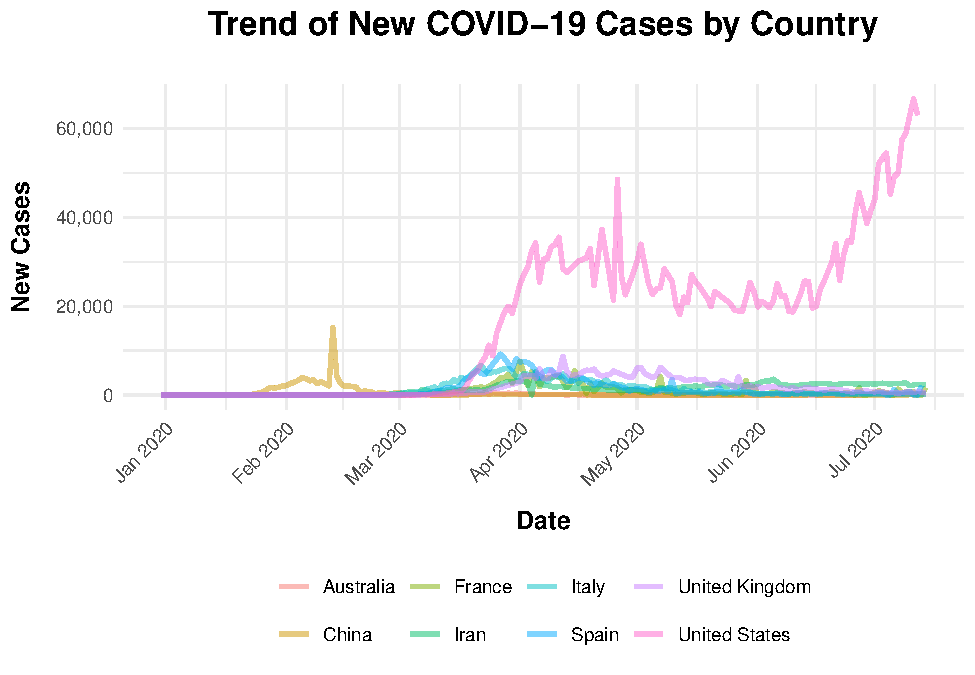
\includegraphics{Part_A_Covid_files/figure-latex/line-plot-1.pdf}

The first occurrence of a notable observation of new cases is in China,
which reflects the fact that it is the origin of the novel coronavirus
outbreak, also known as COVID-19 (Centers for Disease Control and
Prevention (2024)). A significant increase can also be seen in the
United States, compared to other countries in the dataset, which started
after about a month since China's spike. This event forced a declaration
in the United States for a nationwide emergency and further overseas
travel bans on the 13th of March, 2020. (Centers for Disease Control and
Prevention (2024)). By August 2020, the reported total number of cases
in U.S.A. was 5.04 million, which is evident of the prolonged large
number of new cases daily as seen in the plot (Bergquist et al. (2020)).

Apart from the two significant findings previously mentioned, it can
also be seen that the trend of the number of new cases are similar among
the European countries. By February 2020, the virus has reached Europe,
with Italy being the first to react with lockdowns in different
provinces as cases began to rise. By April 2020, numerous countries in
Europe have reached 10,000 total cases, which is also evident in the
plot (Chadwick (2020))

The observed shift in the increase of new cases from China to other
countries supports the fact that the outbreak originated in China. As
international travel occurs daily, the spread of the virus to other
places was inevitable, which explains the gradual and fluctuating rise
in cases. Because of this, numerous countries implemented lockdowns and
travel bans to control the spread of the virus, leading to a slow
decline in new cases, which became more apparent by the middle to late
part of 2020 in most countries. \vspace{1cm}

Now here is an observation of the relationship between the death rate
and new case numbers with the GDP of each country.

\begin{Shaded}
\begin{Highlighting}[]
\NormalTok{mean\_gdp }\OtherTok{\textless{}{-}}\NormalTok{ data }\SpecialCharTok{\%\textgreater{}\%}
  \FunctionTok{summarise}\NormalTok{(}\AttributeTok{mean\_gdp =} \FunctionTok{mean}\NormalTok{(gdp\_per\_capita, }\AttributeTok{na.rm =} \ConstantTok{TRUE}\NormalTok{)) }\SpecialCharTok{\%\textgreater{}\%}
  \FunctionTok{pull}\NormalTok{(mean\_gdp)}
\FunctionTok{cat}\NormalTok{(}\StringTok{"Mean GDP: "}\NormalTok{, mean\_gdp, }\StringTok{"}\SpecialCharTok{\textbackslash{}n}\StringTok{"}\NormalTok{)}
\end{Highlighting}
\end{Shaded}

\begin{verbatim}
## Mean GDP:  27512.46
\end{verbatim}

\begin{Shaded}
\begin{Highlighting}[]
\NormalTok{data }\OtherTok{\textless{}{-}}\NormalTok{ data }\SpecialCharTok{\%\textgreater{}\%}
  \FunctionTok{mutate}\NormalTok{(}\AttributeTok{GDP\_Status =} \FunctionTok{ifelse}\NormalTok{(gdp\_per\_capita }\SpecialCharTok{\textgreater{}=}\NormalTok{ mean\_gdp, }\DecValTok{1}\NormalTok{, }\DecValTok{0}\NormalTok{))}

\FunctionTok{cat}\NormalTok{(}\StringTok{"Number of rows with GDP Status 1: "}\NormalTok{, }\FunctionTok{nrow}\NormalTok{(data[data}\SpecialCharTok{$}\NormalTok{GDP\_Status }\SpecialCharTok{==} \DecValTok{1}\NormalTok{, ]), }\StringTok{"}\SpecialCharTok{\textbackslash{}n}\StringTok{"}\NormalTok{)}
\FunctionTok{cat}\NormalTok{(}\StringTok{"Number of rows with GDP Status 0: "}\NormalTok{, }\FunctionTok{nrow}\NormalTok{(data[data}\SpecialCharTok{$}\NormalTok{GDP\_Status }\SpecialCharTok{==} \DecValTok{0}\NormalTok{, ]), }\StringTok{"}\SpecialCharTok{\textbackslash{}n}\StringTok{"}\NormalTok{)}
\end{Highlighting}
\end{Shaded}

\begin{verbatim}
## Number of rows with GDP Status 1 (GDP greater than or equal to the mean):  5861
\end{verbatim}

\begin{verbatim}
## Number of rows with GDP Status 0 (GDP less than the mean):  6442
\end{verbatim}

\begin{Shaded}
\begin{Highlighting}[]
\NormalTok{data }\OtherTok{\textless{}{-}}\NormalTok{ data }\SpecialCharTok{\%\textgreater{}\%}
  \FunctionTok{mutate}\NormalTok{(}\AttributeTok{new\_case\_rate =}\NormalTok{ new\_cases }\SpecialCharTok{/}\NormalTok{ population,}
         \AttributeTok{new\_death\_rate =}\NormalTok{ new\_deaths }\SpecialCharTok{/}\NormalTok{ population)}

\FunctionTok{head}\NormalTok{(data }\SpecialCharTok{\%\textgreater{}\%} \FunctionTok{filter}\NormalTok{(new\_case\_rate }\SpecialCharTok{\textgreater{}} \DecValTok{0} \SpecialCharTok{\&}\NormalTok{ new\_death\_rate }\SpecialCharTok{\textgreater{}} \DecValTok{0}\NormalTok{), }\DecValTok{10}\NormalTok{)}
\end{Highlighting}
\end{Shaded}

\begin{verbatim}
##     location       date total_cases new_cases total_deaths new_deaths
## 1  Australia 2020-03-01          26         1            1          1
## 2  Australia 2020-03-01          26         1            1          1
## 3  Australia 2020-03-01          26         1            1          1
## 4  Australia 2020-03-01          26         1            1          1
## 5  Australia 2020-03-01          26         1            1          1
## 6  Australia 2020-03-01          26         1            1          1
## 7  Australia 2020-03-01          26         1            1          1
## 8  Australia 2020-03-01          26         1            1          1
## 9  Australia 2020-03-05          52        11            2          1
## 10 Australia 2020-03-05          52        11            2          1
##    gdp_per_capita population lockdown_date total doses administered
## 1        44648.71   25499881          <NA>                 57988175
## 2        44648.71   25499881          <NA>                 57988175
## 3        44648.71   25499881          <NA>                 57988175
## 4        44648.71   25499881          <NA>                 57988175
## 5        44648.71   25499881          <NA>                 57988175
## 6        44648.71   25499881          <NA>                 57988175
## 7        44648.71   25499881    2020-03-24                 57988175
## 8        44648.71   25499881          <NA>                 57988175
## 9        44648.71   25499881          <NA>                 57988175
## 10       44648.71   25499881          <NA>                 57988175
##    % of population fully vaccinated GDP_Status new_case_rate new_death_rate
## 1                                86          1  3.921587e-08   3.921587e-08
## 2                                86          1  3.921587e-08   3.921587e-08
## 3                                86          1  3.921587e-08   3.921587e-08
## 4                                86          1  3.921587e-08   3.921587e-08
## 5                                86          1  3.921587e-08   3.921587e-08
## 6                                86          1  3.921587e-08   3.921587e-08
## 7                                86          1  3.921587e-08   3.921587e-08
## 8                                86          1  3.921587e-08   3.921587e-08
## 9                                86          1  4.313746e-07   3.921587e-08
## 10                               86          1  4.313746e-07   3.921587e-08
\end{verbatim}

\begin{Shaded}
\begin{Highlighting}[]
\FunctionTok{ggplot}\NormalTok{(data, }\FunctionTok{aes}\NormalTok{(}\AttributeTok{x =}\NormalTok{ new\_case\_rate, }\AttributeTok{y =}\NormalTok{ new\_death\_rate, }\AttributeTok{color =} \FunctionTok{factor}\NormalTok{(GDP\_Status))) }\SpecialCharTok{+}
  \FunctionTok{geom\_point}\NormalTok{(}\AttributeTok{alpha =} \FloatTok{0.7}\NormalTok{) }\SpecialCharTok{+}
  \FunctionTok{scale\_color\_manual}\NormalTok{(}
    \AttributeTok{values =} \FunctionTok{c}\NormalTok{(}\StringTok{"0"} \OtherTok{=} \StringTok{"firebrick"}\NormalTok{, }\StringTok{"1"} \OtherTok{=} \StringTok{"steelblue"}\NormalTok{),}
    \AttributeTok{labels =} \FunctionTok{c}\NormalTok{(}\StringTok{"0"} \OtherTok{=} \StringTok{"Less than average"}\NormalTok{, }\StringTok{"1"} \OtherTok{=} \StringTok{"Equal to or greater than average"}\NormalTok{),}
    \AttributeTok{name =} \StringTok{"GDP Category"}
\NormalTok{  ) }\SpecialCharTok{+}
  \FunctionTok{labs}\NormalTok{(}
    \AttributeTok{title =} \StringTok{"Daily Case and Death Rate by GDP Status"}\NormalTok{,}
    \AttributeTok{x =} \StringTok{"Daily Case Rate"}\NormalTok{,}
    \AttributeTok{y =} \StringTok{"Daily Death Rate"}
\NormalTok{  ) }\SpecialCharTok{+}
  \FunctionTok{theme\_minimal}\NormalTok{()}
\end{Highlighting}
\end{Shaded}

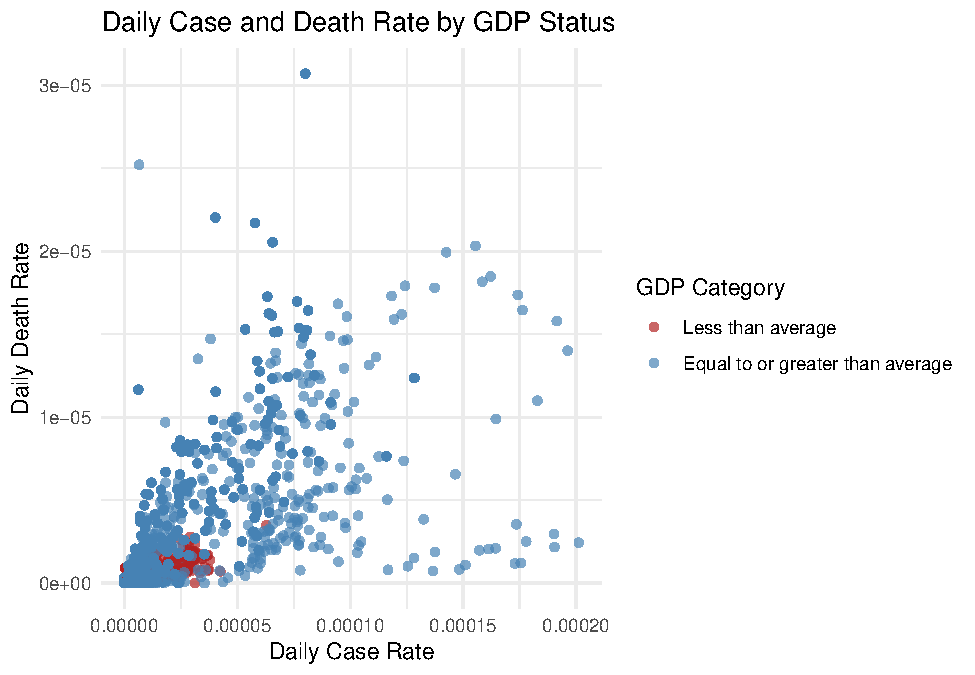
\includegraphics{Part_A_Covid_files/figure-latex/scatter-plot-new-case-death-rate-1.pdf}

The Gross Domestic Product, or GDP, is a representation of the monetary
value of goods and services produced by a country in a specified period.
(Callen (2025)) If this value is to be divided by the total population
of a country, we would get the GDP per capita, which is the number that
we have in our dataset that represents a rough measure of a country's
living standards, or simply, the financial capability of a person in the
country.

From the scatter plot above, it can be seen that countries with lower
than average GDP per capita tend to have lower daily new/death case
rates. This can be due to multiple factors such as the country lacking
the capability to have robust healthcare and data systems, leading to
underreporting of the number of new cases and deaths per day. It can
also be linked to factors such as the life expectancy and tourist
spending being significantly lower than those that have average or
greater GDP per capita. To provide an example:

\begin{itemize}
\tightlist
\item
  Luxembourg is identified as having the highest GDP per capita. Burundi
  is identified as having the lowest estimated GDP per capita. (The
  World Factbook (2025)).\newline
\item
  Life expectancy in Luxembourg is 82.8 years. Burundi's is 64 years.
  Almost 20 years difference (World Health Organisation, 2023).\newline
\item
  Luxembourg tourist spending for 2017 was 5.47 billion US Dollars
  (macrotrends (2025)). Burundi tourist spending for 2017 was 0.1
  billion US dollars. (Knoema Data Appliance (2025)).
\end{itemize}

Overseas travel played a major role in the global spread of COVID-19 as
rapid transmission across borders occurred. In 2020, the death rate from
the virus for those that are aged 85 and over was 1,645 per 100,000
population -- seven times greater than the rate for those aged 65 to 74.
(Tejada-Vera et al. (2022)).

\section{Predictive Data Analaysis}\label{predictive-data-analaysis}

For this part, I will be fitting a model to make predictions on the
newly infected case and death case numbers for the next five to seven
days. I will be using Polynomial Regression to fit the model for the GDP
group of countries whose GDP per capita is greater than or equal to the
average GDP per capita of all countries in the dataset. This is because
the countries in the group have daily new cases and deaths that are more
spread out, which is more suitable for training a model since the data
is more varied.

Firstly, let's create the model so we can plot a polynomial regression
line. I will start with using the number of days since the earliest date
in the dataset as the predictor variable for the number of new cases.
For the training and testing sets, I will split the data into 70\% for
training and 30\% for testing.

\begin{Shaded}
\begin{Highlighting}[]
\NormalTok{data\_higher\_gdp }\OtherTok{\textless{}{-}}\NormalTok{ data }\SpecialCharTok{\%\textgreater{}\%}
  \FunctionTok{filter}\NormalTok{(GDP\_Status }\SpecialCharTok{==} \DecValTok{1}\NormalTok{, }\SpecialCharTok{!}\FunctionTok{is.na}\NormalTok{(new\_cases), }\SpecialCharTok{!}\FunctionTok{is.na}\NormalTok{(date)) }\SpecialCharTok{\%\textgreater{}\%}
  \FunctionTok{mutate}\NormalTok{(}\AttributeTok{date\_num =} \FunctionTok{as.numeric}\NormalTok{(}\FunctionTok{as.Date}\NormalTok{(date) }\SpecialCharTok{{-}} \FunctionTok{min}\NormalTok{(}\FunctionTok{as.Date}\NormalTok{(date))))}

\CommentTok{\# Split train/test sets}
\FunctionTok{set.seed}\NormalTok{(}\DecValTok{4}\NormalTok{)}
\NormalTok{train\_indices }\OtherTok{\textless{}{-}} \FunctionTok{sample}\NormalTok{(}\DecValTok{1}\SpecialCharTok{:}\FunctionTok{nrow}\NormalTok{(data\_higher\_gdp), }\AttributeTok{size =} \FloatTok{0.7} \SpecialCharTok{*} \FunctionTok{nrow}\NormalTok{(data\_higher\_gdp))}
\NormalTok{train }\OtherTok{\textless{}{-}}\NormalTok{ data\_higher\_gdp[train\_indices, ]}
\NormalTok{test }\OtherTok{\textless{}{-}}\NormalTok{ data\_higher\_gdp[}\SpecialCharTok{{-}}\NormalTok{train\_indices, ]}

\CommentTok{\# Create a sequence of dates for smooth prediction lines}
\NormalTok{date\_seq }\OtherTok{\textless{}{-}} \FunctionTok{seq}\NormalTok{(}\FunctionTok{min}\NormalTok{(train}\SpecialCharTok{$}\NormalTok{date\_num), }\FunctionTok{max}\NormalTok{(train}\SpecialCharTok{$}\NormalTok{date\_num), }\AttributeTok{length.out =} \DecValTok{100}\NormalTok{)}

\CommentTok{\# Initialize a dataframe to store predictions for all models}
\NormalTok{all\_preds }\OtherTok{\textless{}{-}} \FunctionTok{data.frame}\NormalTok{()}

\ControlFlowTok{for}\NormalTok{ (deg }\ControlFlowTok{in} \DecValTok{1}\SpecialCharTok{:}\DecValTok{10}\NormalTok{) \{}
  \CommentTok{\# Fit the model with current degree for date}
\NormalTok{  model }\OtherTok{\textless{}{-}} \FunctionTok{lm}\NormalTok{(new\_cases }\SpecialCharTok{\textasciitilde{}} \FunctionTok{poly}\NormalTok{(date\_num, deg), }\AttributeTok{data =}\NormalTok{ train)}
  
  \CommentTok{\# Predict on the date sequence with fixed GDP per capita}
\NormalTok{  pred\_df }\OtherTok{\textless{}{-}} \FunctionTok{data.frame}\NormalTok{(}\AttributeTok{date\_num =}\NormalTok{ date\_seq)}
\NormalTok{  pred\_df}\SpecialCharTok{$}\NormalTok{new\_cases }\OtherTok{\textless{}{-}} \FunctionTok{predict}\NormalTok{(model, }\AttributeTok{newdata =}\NormalTok{ pred\_df)}
\NormalTok{  pred\_df}\SpecialCharTok{$}\NormalTok{degree }\OtherTok{\textless{}{-}} \FunctionTok{factor}\NormalTok{(deg)}
  
\NormalTok{  all\_preds }\OtherTok{\textless{}{-}} \FunctionTok{bind\_rows}\NormalTok{(all\_preds, pred\_df)}
\NormalTok{\}}

\CommentTok{\# Plot all polynomial lines in a facet grid}
\FunctionTok{ggplot}\NormalTok{() }\SpecialCharTok{+}
  \FunctionTok{geom\_point}\NormalTok{(}\AttributeTok{data =}\NormalTok{ train, }\FunctionTok{aes}\NormalTok{(}\AttributeTok{x =}\NormalTok{ date\_num, }\AttributeTok{y =}\NormalTok{ new\_cases), }\AttributeTok{alpha =} \FloatTok{0.3}\NormalTok{) }\SpecialCharTok{+}
  \FunctionTok{geom\_line}\NormalTok{(}\AttributeTok{data =}\NormalTok{ all\_preds, }\FunctionTok{aes}\NormalTok{(}\AttributeTok{x =}\NormalTok{ date\_num, }\AttributeTok{y =}\NormalTok{ new\_cases, }\AttributeTok{color =}\NormalTok{ degree), }\AttributeTok{size =} \DecValTok{1}\NormalTok{) }\SpecialCharTok{+}
  \FunctionTok{facet\_wrap}\NormalTok{(}\SpecialCharTok{\textasciitilde{}}\NormalTok{ degree, }\AttributeTok{scales =} \StringTok{"free\_x"}\NormalTok{) }\SpecialCharTok{+}
  \FunctionTok{labs}\NormalTok{(}
    \AttributeTok{title =} \StringTok{"Polynomial Regression Lines for Different Degrees (New Cases)"}\NormalTok{,}
    \AttributeTok{x =} \StringTok{"Date (in days since start)"}\NormalTok{,}
    \AttributeTok{y =} \StringTok{"New Cases"}
\NormalTok{  ) }\SpecialCharTok{+}
  \FunctionTok{theme\_minimal}\NormalTok{()}
\end{Highlighting}
\end{Shaded}

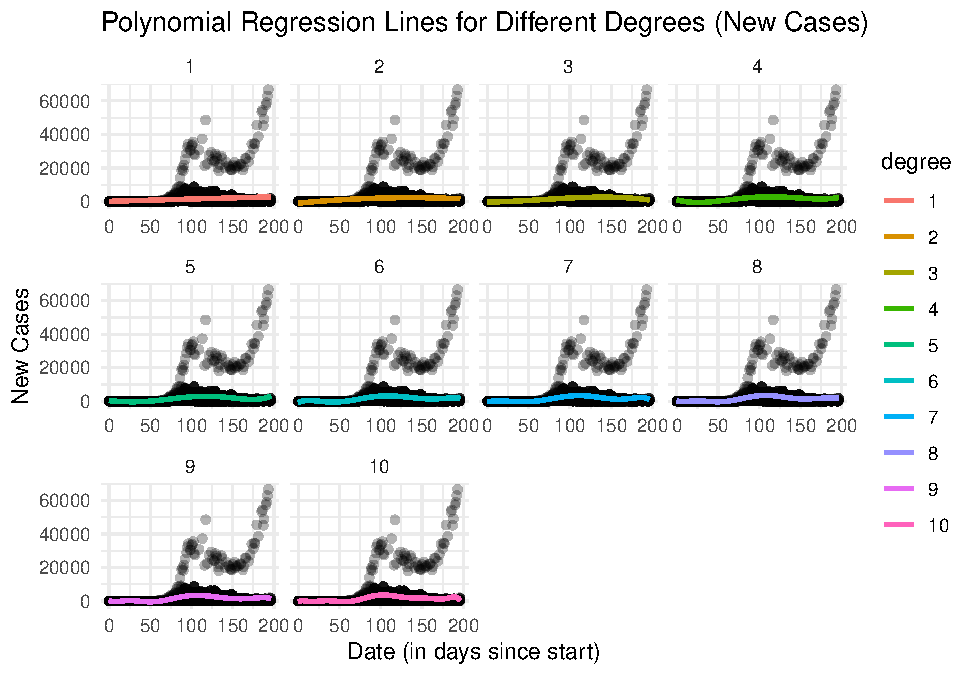
\includegraphics{Part_A_Covid_files/figure-latex/polynomial-regression-date-1.pdf}
From these plots, I can see that, the polynomial regression lines for
all of the degrees don't seem to have much differences and all seem to
be a good fit. However, I will choose the degree 5 as it seems to be a
good balance between complexity and fit, without overfitting the data.
\vspace{1cm}

Next, I will use the total number of cases as the predictor variable.

\begin{Shaded}
\begin{Highlighting}[]
\CommentTok{\# Model to predict new cases based on total cases}
\NormalTok{all\_preds }\OtherTok{\textless{}{-}} \FunctionTok{data.frame}\NormalTok{()  }\CommentTok{\# initialize outside the loop}

\ControlFlowTok{for}\NormalTok{ (deg }\ControlFlowTok{in} \DecValTok{1}\SpecialCharTok{:}\DecValTok{10}\NormalTok{) \{}
\NormalTok{  model }\OtherTok{\textless{}{-}} \FunctionTok{lm}\NormalTok{(new\_cases }\SpecialCharTok{\textasciitilde{}} \FunctionTok{poly}\NormalTok{(total\_cases, deg), }\AttributeTok{data =}\NormalTok{ train)}
  
\NormalTok{  pred\_df }\OtherTok{\textless{}{-}} \FunctionTok{data.frame}\NormalTok{(}\AttributeTok{total\_cases =} \FunctionTok{seq}\NormalTok{(}\FunctionTok{min}\NormalTok{(train}\SpecialCharTok{$}\NormalTok{total\_cases), }\FunctionTok{max}\NormalTok{(train}\SpecialCharTok{$}\NormalTok{total\_cases), }\AttributeTok{length.out =} \DecValTok{100}\NormalTok{))}
\NormalTok{  pred\_df}\SpecialCharTok{$}\NormalTok{new\_cases }\OtherTok{\textless{}{-}} \FunctionTok{predict}\NormalTok{(model, }\AttributeTok{newdata =}\NormalTok{ pred\_df)}
\NormalTok{  pred\_df}\SpecialCharTok{$}\NormalTok{degree }\OtherTok{\textless{}{-}} \FunctionTok{factor}\NormalTok{(deg)}
  
\NormalTok{  all\_preds }\OtherTok{\textless{}{-}} \FunctionTok{bind\_rows}\NormalTok{(all\_preds, pred\_df)}
\NormalTok{\}}

\FunctionTok{ggplot}\NormalTok{() }\SpecialCharTok{+}
  \FunctionTok{geom\_point}\NormalTok{(}\AttributeTok{data =}\NormalTok{ train, }\FunctionTok{aes}\NormalTok{(}\AttributeTok{x =}\NormalTok{ total\_cases, }\AttributeTok{y =}\NormalTok{ new\_cases), }\AttributeTok{alpha =} \FloatTok{0.3}\NormalTok{) }\SpecialCharTok{+}
  \FunctionTok{geom\_line}\NormalTok{(}\AttributeTok{data =}\NormalTok{ all\_preds, }\FunctionTok{aes}\NormalTok{(}\AttributeTok{x =}\NormalTok{ total\_cases, }\AttributeTok{y =}\NormalTok{ new\_cases, }\AttributeTok{color =}\NormalTok{ degree), }\AttributeTok{size =} \DecValTok{1}\NormalTok{) }\SpecialCharTok{+}
  \FunctionTok{facet\_wrap}\NormalTok{(}\SpecialCharTok{\textasciitilde{}}\NormalTok{ degree, }\AttributeTok{scales =} \StringTok{"free\_x"}\NormalTok{) }\SpecialCharTok{+}
  \FunctionTok{labs}\NormalTok{(}
    \AttributeTok{title =} \StringTok{"Polynomial Regression Lines for Different Degrees (Total Cases)"}\NormalTok{,}
    \AttributeTok{x =} \StringTok{"Total Cases"}\NormalTok{,}
    \AttributeTok{y =} \StringTok{"New Cases"}
\NormalTok{  ) }\SpecialCharTok{+}
  \FunctionTok{theme\_minimal}\NormalTok{()}
\end{Highlighting}
\end{Shaded}

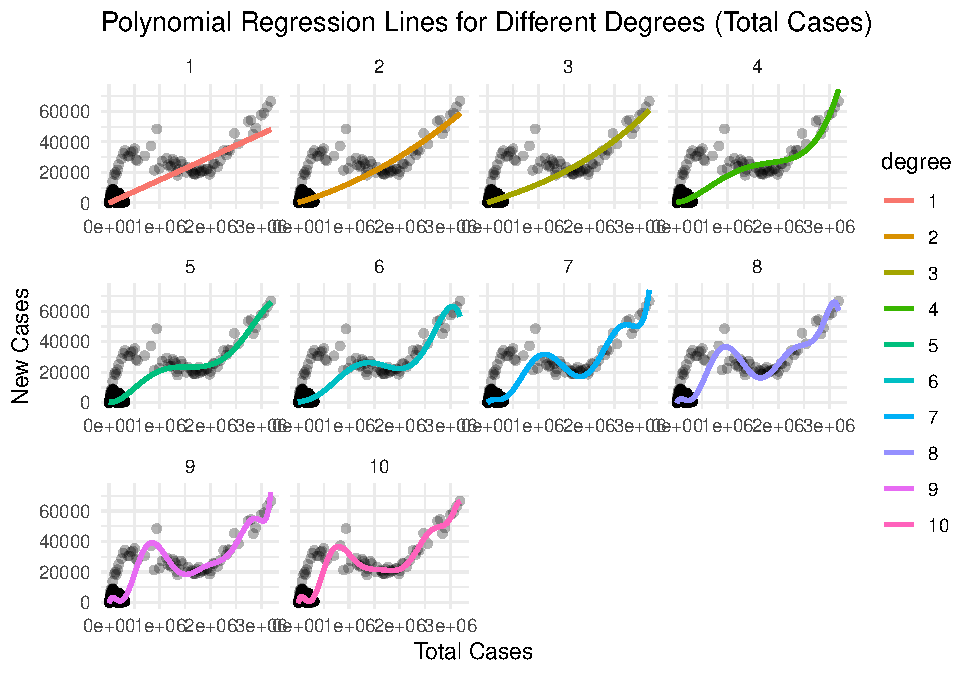
\includegraphics{Part_A_Covid_files/figure-latex/polynomial-regression-total-cases-1.pdf}
From these plots, I can see that degree 7 seems to be the best fit for
the polynomial regression line, as it captures the trend of the new
cases based on the total cases without overfitting. \vspace{1cm}

Next, I want to check what other variables can be used to predict the
new cases. The three variables below are the ones that might have an
effect on the number of new cases. I will check the number of unique
values in each of these variables to see if they are suitable for
polynomial regression.

\begin{verbatim}
## number of unique locations in the dataset:  6
\end{verbatim}

\begin{verbatim}
## number of unique population values in the dataset:  6
\end{verbatim}

\begin{verbatim}
## number of unique GDP per capita values in the dataset:  6
\end{verbatim}

There are six unique locations, unique population values and unique GDP
per capita values in the dataset. Six different locations might be a
good number to use as a predictor variable. Six unique population values
most likely isn't enough to use as a predictor variable, given that the
population value is numerical. Similarly, six unique GDP per capita
values is also not enough to use as a predictor variable.

I will now use the location as a predictor variable for the new cases.

\begin{Shaded}
\begin{Highlighting}[]
\CommentTok{\# Convert location to a factor}
\NormalTok{data\_higher\_gdp}\SpecialCharTok{$}\NormalTok{location }\OtherTok{\textless{}{-}} \FunctionTok{as.factor}\NormalTok{(data\_higher\_gdp}\SpecialCharTok{$}\NormalTok{location)}
\NormalTok{train}\SpecialCharTok{$}\NormalTok{location }\OtherTok{\textless{}{-}} \FunctionTok{as.factor}\NormalTok{(train}\SpecialCharTok{$}\NormalTok{location)}
\NormalTok{test}\SpecialCharTok{$}\NormalTok{location }\OtherTok{\textless{}{-}} \FunctionTok{as.factor}\NormalTok{(test}\SpecialCharTok{$}\NormalTok{location)}

\CommentTok{\# Create a sequence of locations for smooth prediction lines}
\NormalTok{location\_seq }\OtherTok{\textless{}{-}} \FunctionTok{levels}\NormalTok{(data\_higher\_gdp}\SpecialCharTok{$}\NormalTok{location)}

\CommentTok{\# Initialize a dataframe to store predictions for all models}
\NormalTok{all\_preds }\OtherTok{\textless{}{-}} \FunctionTok{data.frame}\NormalTok{()}

\ControlFlowTok{for}\NormalTok{ (deg }\ControlFlowTok{in} \DecValTok{1}\SpecialCharTok{:}\DecValTok{5}\NormalTok{) \{}
  \CommentTok{\# Fit the model with current degree for location}
\NormalTok{  model }\OtherTok{\textless{}{-}} \FunctionTok{lm}\NormalTok{(new\_cases }\SpecialCharTok{\textasciitilde{}} \FunctionTok{poly}\NormalTok{(}\FunctionTok{as.numeric}\NormalTok{(location), deg), }\AttributeTok{data =}\NormalTok{ train)}
  
  \CommentTok{\# Predict on the location sequence}
\NormalTok{  pred\_df }\OtherTok{\textless{}{-}} \FunctionTok{data.frame}\NormalTok{(}\AttributeTok{location =} \FunctionTok{seq\_along}\NormalTok{(location\_seq))}
\NormalTok{  pred\_df}\SpecialCharTok{$}\NormalTok{new\_cases }\OtherTok{\textless{}{-}} \FunctionTok{predict}\NormalTok{(model, }\AttributeTok{newdata =}\NormalTok{ pred\_df)}
\NormalTok{  pred\_df}\SpecialCharTok{$}\NormalTok{degree }\OtherTok{\textless{}{-}} \FunctionTok{factor}\NormalTok{(deg)}
  
\NormalTok{  all\_preds }\OtherTok{\textless{}{-}} \FunctionTok{bind\_rows}\NormalTok{(all\_preds, pred\_df)}
\NormalTok{\}}

\CommentTok{\# Plot all polynomial lines in a facet grid}
\FunctionTok{ggplot}\NormalTok{() }\SpecialCharTok{+}
  \FunctionTok{geom\_point}\NormalTok{(}\AttributeTok{data =}\NormalTok{ train, }\FunctionTok{aes}\NormalTok{(}\AttributeTok{x =} \FunctionTok{as.numeric}\NormalTok{(location), }\AttributeTok{y =}\NormalTok{ new\_cases), }\AttributeTok{alpha =} \FloatTok{0.3}\NormalTok{) }\SpecialCharTok{+}
  \FunctionTok{geom\_line}\NormalTok{(}\AttributeTok{data =}\NormalTok{ all\_preds, }\FunctionTok{aes}\NormalTok{(}\AttributeTok{x =} \FunctionTok{as.numeric}\NormalTok{(location), }\AttributeTok{y =}\NormalTok{ new\_cases, }\AttributeTok{color =}\NormalTok{ degree), }\AttributeTok{size =} \DecValTok{1}\NormalTok{) }\SpecialCharTok{+}
  \FunctionTok{facet\_wrap}\NormalTok{(}\SpecialCharTok{\textasciitilde{}}\NormalTok{ degree, }\AttributeTok{scales =} \StringTok{"free\_x"}\NormalTok{) }\SpecialCharTok{+}
  \FunctionTok{labs}\NormalTok{(}
    \AttributeTok{title =} \StringTok{"Polynomial Regression Lines for Different Degrees (New Cases by Location)"}\NormalTok{,}
    \AttributeTok{x =} \StringTok{"Location"}\NormalTok{,}
    \AttributeTok{y =} \StringTok{"New Cases"}
\NormalTok{  ) }\SpecialCharTok{+}
  \FunctionTok{theme\_minimal}\NormalTok{()}
\end{Highlighting}
\end{Shaded}

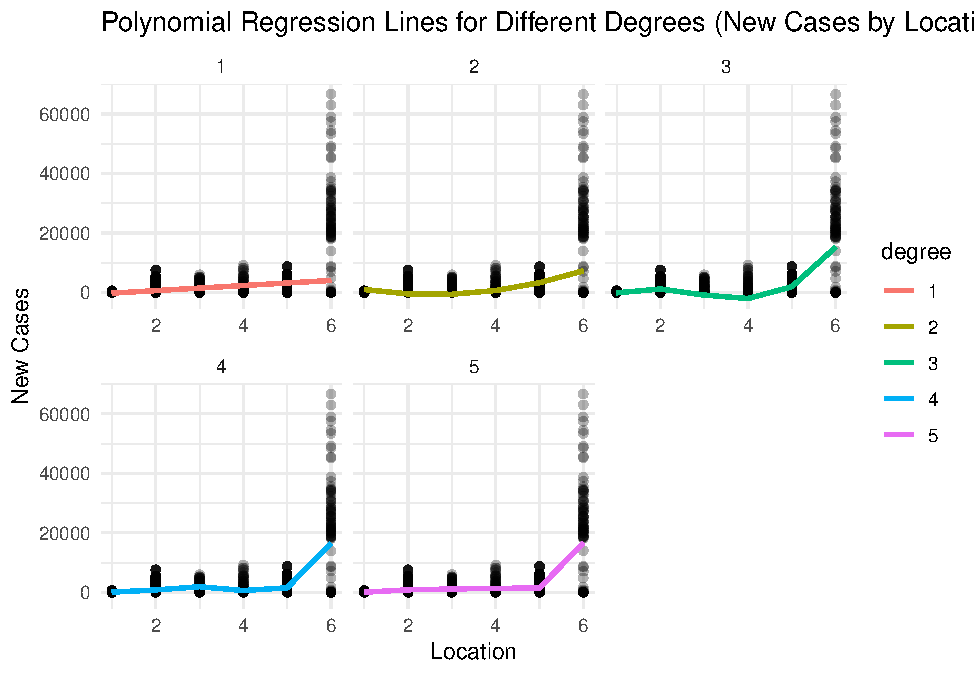
\includegraphics{Part_A_Covid_files/figure-latex/polynomial-regression-location-1.pdf}

\begin{Shaded}
\begin{Highlighting}[]
\CommentTok{\# Print what the encoded locations are}
\NormalTok{location\_encoded }\OtherTok{\textless{}{-}} \FunctionTok{data.frame}\NormalTok{(}
  \AttributeTok{Location =} \FunctionTok{levels}\NormalTok{(data\_higher\_gdp}\SpecialCharTok{$}\NormalTok{location),}
  \AttributeTok{Encoding =} \FunctionTok{seq\_along}\NormalTok{(}\FunctionTok{levels}\NormalTok{(data\_higher\_gdp}\SpecialCharTok{$}\NormalTok{location))}
\NormalTok{)}

\FunctionTok{print}\NormalTok{(location\_encoded)}
\end{Highlighting}
\end{Shaded}

\begin{verbatim}
##         Location Encoding
## 1      Australia        1
## 2         France        2
## 3          Italy        3
## 4          Spain        4
## 5 United Kingdom        5
## 6  United States        6
\end{verbatim}

From these plots, I will chose degree 1 (linear) as it captures the
trend of the new cases based on the location without overfitting.
\vspace{1cm}

Finally, I will now create a model to predict new cases based on the
three predictor variables that I have used and the degrees that are best
suited for each of them. I understand that my choices for the degrees
are subjective to models with only the corresponding predcitor variable
above. Hence, I will loop through the degrees 5, 6, and 7 for the
date\_num and total\_cases predictor variables to see how the line fits
the data.

\begin{Shaded}
\begin{Highlighting}[]
\CommentTok{\# Define the degree combinations for poly(date\_num, deg1) and poly(total\_cases, deg2)}
\NormalTok{deg\_combinations }\OtherTok{\textless{}{-}} \FunctionTok{expand.grid}\NormalTok{(}\AttributeTok{deg\_date =} \DecValTok{5}\SpecialCharTok{:}\DecValTok{7}\NormalTok{, }\AttributeTok{deg\_cases =} \DecValTok{5}\SpecialCharTok{:}\DecValTok{7}\NormalTok{)}

\CommentTok{\# Create prediction dataframe with 100 points}
\NormalTok{date\_seq }\OtherTok{\textless{}{-}} \FunctionTok{seq}\NormalTok{(}\FunctionTok{min}\NormalTok{(train}\SpecialCharTok{$}\NormalTok{date\_num), }\FunctionTok{max}\NormalTok{(train}\SpecialCharTok{$}\NormalTok{date\_num), }\AttributeTok{length.out =} \DecValTok{100}\NormalTok{)}
\NormalTok{mean\_total\_cases }\OtherTok{\textless{}{-}} \FunctionTok{mean}\NormalTok{(train}\SpecialCharTok{$}\NormalTok{total\_cases, }\AttributeTok{na.rm =} \ConstantTok{TRUE}\NormalTok{)}
\NormalTok{fixed\_location }\OtherTok{\textless{}{-}} \FunctionTok{factor}\NormalTok{(}\FunctionTok{levels}\NormalTok{(train}\SpecialCharTok{$}\NormalTok{location)[}\DecValTok{1}\NormalTok{], }\AttributeTok{levels =} \FunctionTok{levels}\NormalTok{(train}\SpecialCharTok{$}\NormalTok{location))}

\CommentTok{\# Container to store all prediction results}
\NormalTok{all\_preds }\OtherTok{\textless{}{-}} \FunctionTok{data.frame}\NormalTok{()}

\CommentTok{\# Loop over all combinations of degrees}
\ControlFlowTok{for}\NormalTok{ (i }\ControlFlowTok{in} \DecValTok{1}\SpecialCharTok{:}\FunctionTok{nrow}\NormalTok{(deg\_combinations)) \{}
\NormalTok{  deg\_date }\OtherTok{\textless{}{-}}\NormalTok{ deg\_combinations}\SpecialCharTok{$}\NormalTok{deg\_date[i]}
\NormalTok{  deg\_cases }\OtherTok{\textless{}{-}}\NormalTok{ deg\_combinations}\SpecialCharTok{$}\NormalTok{deg\_cases[i]}
  
  \CommentTok{\# Fit model}
\NormalTok{  model }\OtherTok{\textless{}{-}} \FunctionTok{lm}\NormalTok{(new\_cases }\SpecialCharTok{\textasciitilde{}} \FunctionTok{poly}\NormalTok{(date\_num, deg\_date) }\SpecialCharTok{+} \FunctionTok{poly}\NormalTok{(total\_cases, deg\_cases) }\SpecialCharTok{+}\NormalTok{ location, }\AttributeTok{data =}\NormalTok{ train)}
  
  \CommentTok{\# Create prediction dataframe}
\NormalTok{  pred\_df }\OtherTok{\textless{}{-}} \FunctionTok{data.frame}\NormalTok{(}
    \AttributeTok{date\_num =}\NormalTok{ date\_seq,}
    \AttributeTok{total\_cases =}\NormalTok{ mean\_total\_cases,}
    \AttributeTok{location =}\NormalTok{ fixed\_location}
\NormalTok{  )}
  
  \CommentTok{\# Predict new cases}
\NormalTok{  pred\_df}\SpecialCharTok{$}\NormalTok{new\_cases }\OtherTok{\textless{}{-}} \FunctionTok{predict}\NormalTok{(model, }\AttributeTok{newdata =}\NormalTok{ pred\_df)}
\NormalTok{  pred\_df}\SpecialCharTok{$}\NormalTok{deg\_date\_num }\OtherTok{\textless{}{-}} \FunctionTok{factor}\NormalTok{(deg\_date)}
\NormalTok{  pred\_df}\SpecialCharTok{$}\NormalTok{deg\_total\_cases }\OtherTok{\textless{}{-}} \FunctionTok{factor}\NormalTok{(deg\_cases)}
  
\NormalTok{  all\_preds }\OtherTok{\textless{}{-}} \FunctionTok{bind\_rows}\NormalTok{(all\_preds, pred\_df)}
\NormalTok{\}}

\CommentTok{\# Plot: Facet grid of regression lines}
\FunctionTok{ggplot}\NormalTok{() }\SpecialCharTok{+}
  \FunctionTok{geom\_point}\NormalTok{(}\AttributeTok{data =}\NormalTok{ train, }\FunctionTok{aes}\NormalTok{(}\AttributeTok{x =}\NormalTok{ date\_num, }\AttributeTok{y =}\NormalTok{ new\_cases), }\AttributeTok{alpha =} \FloatTok{0.2}\NormalTok{) }\SpecialCharTok{+}
  \FunctionTok{geom\_line}\NormalTok{(}\AttributeTok{data =}\NormalTok{ all\_preds, }\FunctionTok{aes}\NormalTok{(}\AttributeTok{x =}\NormalTok{ date\_num, }\AttributeTok{y =}\NormalTok{ new\_cases, }\AttributeTok{color =}\NormalTok{ deg\_total\_cases), }\AttributeTok{size =} \DecValTok{1}\NormalTok{) }\SpecialCharTok{+}
  \FunctionTok{facet\_grid}\NormalTok{(deg\_total\_cases }\SpecialCharTok{\textasciitilde{}}\NormalTok{ deg\_date\_num, }\AttributeTok{labeller =}\NormalTok{ label\_both) }\SpecialCharTok{+}
  \FunctionTok{labs}\NormalTok{(}
    \AttributeTok{title =} \StringTok{"Polynomial Regression Lines for Combinations of Degrees"}\NormalTok{,}
    \AttributeTok{x =} \StringTok{"Date (in days since start)"}\NormalTok{,}
    \AttributeTok{y =} \StringTok{"New Cases"}\NormalTok{,}
    \AttributeTok{color =} \StringTok{"Degree"}
\NormalTok{  ) }\SpecialCharTok{+}
  \FunctionTok{theme\_minimal}\NormalTok{()}
\end{Highlighting}
\end{Shaded}

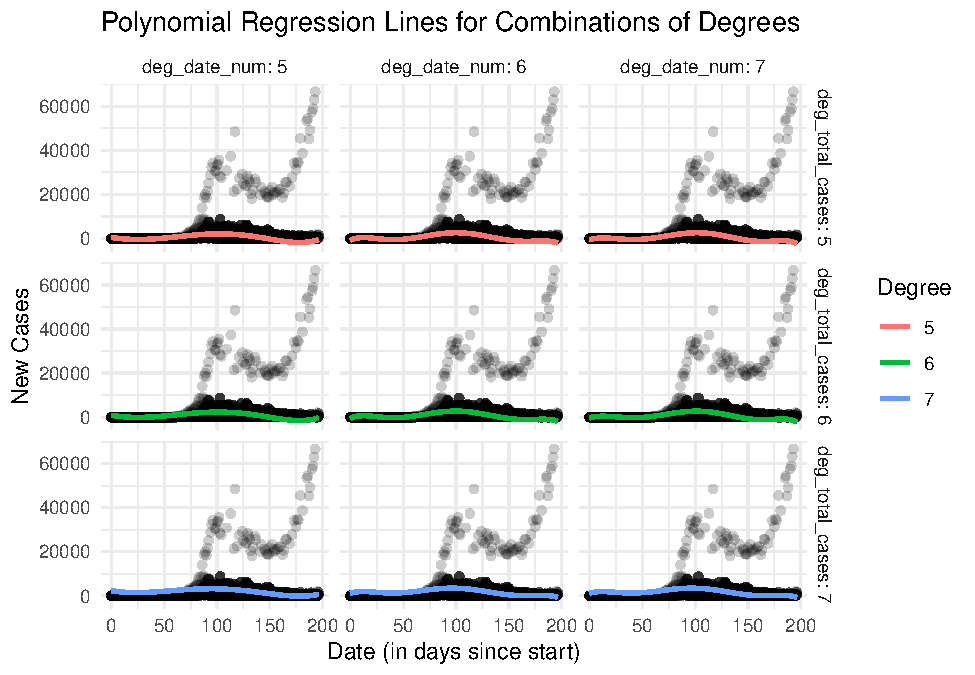
\includegraphics{Part_A_Covid_files/figure-latex/polynomial-regression-deciding-for-final-1.pdf}

From these plots, I can see that the polynomial regression lines for the
combinations of degrees 5, 6, and 7 for date\_num and total\_cases do
not seem to have much differences and all seem to be a good fit.
However, I will choose the combination of degree 5 for date\_num and
degree 6 for total\_cases as it seems to be a good balance between
complexity and fit, without overfitting the data. \vspace{1cm}

Here's the plot for the final model for a better visualisation of the
polynomial regression line.

\begin{Shaded}
\begin{Highlighting}[]
\CommentTok{\# Final model with chosen degrees}
\NormalTok{final\_model }\OtherTok{\textless{}{-}} \FunctionTok{lm}\NormalTok{(new\_cases }\SpecialCharTok{\textasciitilde{}} \FunctionTok{poly}\NormalTok{(date\_num, }\DecValTok{5}\NormalTok{) }\SpecialCharTok{+} \FunctionTok{poly}\NormalTok{(total\_cases, }\DecValTok{6}\NormalTok{) }\SpecialCharTok{+}\NormalTok{ location, }\AttributeTok{data =}\NormalTok{ train)}

\CommentTok{\# Create prediction dataframe}
\NormalTok{pred\_df }\OtherTok{\textless{}{-}} \FunctionTok{data.frame}\NormalTok{(}
  \AttributeTok{date\_num =}\NormalTok{ date\_seq,}
  \AttributeTok{total\_cases =}\NormalTok{ mean\_total\_cases,}
  \AttributeTok{location =}\NormalTok{ fixed\_location}
\NormalTok{)}

\CommentTok{\# Predict new cases}
\NormalTok{pred\_df}\SpecialCharTok{$}\NormalTok{new\_cases }\OtherTok{\textless{}{-}} \FunctionTok{predict}\NormalTok{(final\_model, }\AttributeTok{newdata =}\NormalTok{ pred\_df)}

\CommentTok{\# Plot the final model}
\FunctionTok{ggplot}\NormalTok{() }\SpecialCharTok{+}
  \FunctionTok{geom\_point}\NormalTok{(}\AttributeTok{data =}\NormalTok{ train, }\FunctionTok{aes}\NormalTok{(}\AttributeTok{x =}\NormalTok{ date\_num, }\AttributeTok{y =}\NormalTok{ new\_cases), }\AttributeTok{alpha =} \FloatTok{0.2}\NormalTok{) }\SpecialCharTok{+}
  \FunctionTok{geom\_line}\NormalTok{(}\AttributeTok{data =}\NormalTok{ pred\_df, }\FunctionTok{aes}\NormalTok{(}\AttributeTok{x =}\NormalTok{ date\_num, }\AttributeTok{y =}\NormalTok{ new\_cases), }\AttributeTok{color =} \StringTok{"blue"}\NormalTok{, }\AttributeTok{size =} \DecValTok{1}\NormalTok{) }\SpecialCharTok{+}
  \FunctionTok{labs}\NormalTok{(}
    \AttributeTok{title =} \StringTok{"Final Polynomial Regression Line for New Cases"}\NormalTok{,}
    \AttributeTok{x =} \StringTok{"Date (in days since start)"}\NormalTok{,}
    \AttributeTok{y =} \StringTok{"New Cases"}
\NormalTok{  ) }\SpecialCharTok{+}
  \FunctionTok{theme\_minimal}\NormalTok{()}
\end{Highlighting}
\end{Shaded}

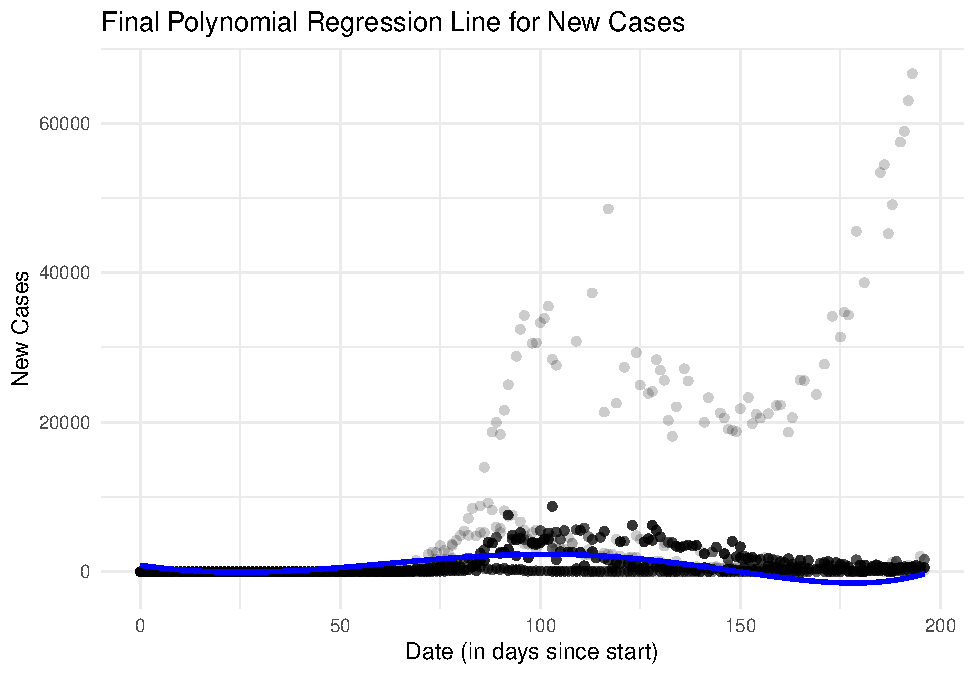
\includegraphics{Part_A_Covid_files/figure-latex/polynomial-regression-final-plot-1.pdf}

\subsubsection{Predictions on the newly infected case
numbers}\label{predictions-on-the-newly-infected-case-numbers}

Now I will use the model to make a prediction on the new cases for the
last five to seven days in the dataset. This is so I can compare the
predicted values with the actual values in the dataset. I will use the
test dataset first, then evaluate using K-fold Cross Validation.

\begin{Shaded}
\begin{Highlighting}[]
\CommentTok{\# Create a prediction dataframe from the test set}
\NormalTok{pred\_test\_df }\OtherTok{\textless{}{-}} \FunctionTok{data.frame}\NormalTok{(}
  \AttributeTok{date\_num =}\NormalTok{ test}\SpecialCharTok{$}\NormalTok{date\_num,}
  \AttributeTok{total\_cases =}\NormalTok{ test}\SpecialCharTok{$}\NormalTok{total\_cases,}
  \AttributeTok{location =}\NormalTok{ test}\SpecialCharTok{$}\NormalTok{location}
\NormalTok{)}

\CommentTok{\# Predict new cases using the final model}
\NormalTok{pred\_test\_df}\SpecialCharTok{$}\NormalTok{predicted\_new\_cases }\OtherTok{\textless{}{-}} \FunctionTok{predict}\NormalTok{(final\_model, }\AttributeTok{newdata =}\NormalTok{ pred\_test\_df)}

\CommentTok{\# Combine with actual test data for comparison}
\NormalTok{test\_combined }\OtherTok{\textless{}{-}}\NormalTok{ test }\SpecialCharTok{\%\textgreater{}\%}
  \FunctionTok{select}\NormalTok{(date\_num, location, new\_cases) }\SpecialCharTok{\%\textgreater{}\%}
  \FunctionTok{mutate}\NormalTok{(}\AttributeTok{predicted\_new\_cases =}\NormalTok{ pred\_test\_df}\SpecialCharTok{$}\NormalTok{predicted\_new\_cases)}

\CommentTok{\# Plot: Actual vs Predicted New Cases on Test Set}
\FunctionTok{ggplot}\NormalTok{(test\_combined, }\FunctionTok{aes}\NormalTok{(}\AttributeTok{x =}\NormalTok{ date\_num)) }\SpecialCharTok{+}
  \FunctionTok{geom\_line}\NormalTok{(}\FunctionTok{aes}\NormalTok{(}\AttributeTok{y =}\NormalTok{ new\_cases, }\AttributeTok{color =} \StringTok{"Actual"}\NormalTok{), }\AttributeTok{size =} \DecValTok{1}\NormalTok{) }\SpecialCharTok{+}
  \FunctionTok{geom\_line}\NormalTok{(}\FunctionTok{aes}\NormalTok{(}\AttributeTok{y =}\NormalTok{ predicted\_new\_cases, }\AttributeTok{color =} \StringTok{"Predicted"}\NormalTok{), }\AttributeTok{size =} \DecValTok{1}\NormalTok{, }\AttributeTok{linetype =} \StringTok{"dashed"}\NormalTok{) }\SpecialCharTok{+}
  \FunctionTok{labs}\NormalTok{(}
    \AttributeTok{title =} \StringTok{"Actual vs Predicted New Cases (Test Set)"}\NormalTok{,}
    \AttributeTok{x =} \StringTok{"Date (in days since start)"}\NormalTok{,}
    \AttributeTok{y =} \StringTok{"New Cases"}\NormalTok{,}
    \AttributeTok{color =} \StringTok{"Legend"}
\NormalTok{  ) }\SpecialCharTok{+}
  \FunctionTok{scale\_color\_manual}\NormalTok{(}\AttributeTok{values =} \FunctionTok{c}\NormalTok{(}\StringTok{"Actual"} \OtherTok{=} \StringTok{"black"}\NormalTok{, }\StringTok{"Predicted"} \OtherTok{=} \StringTok{"blue"}\NormalTok{)) }\SpecialCharTok{+}
  \FunctionTok{theme\_minimal}\NormalTok{()}
\end{Highlighting}
\end{Shaded}

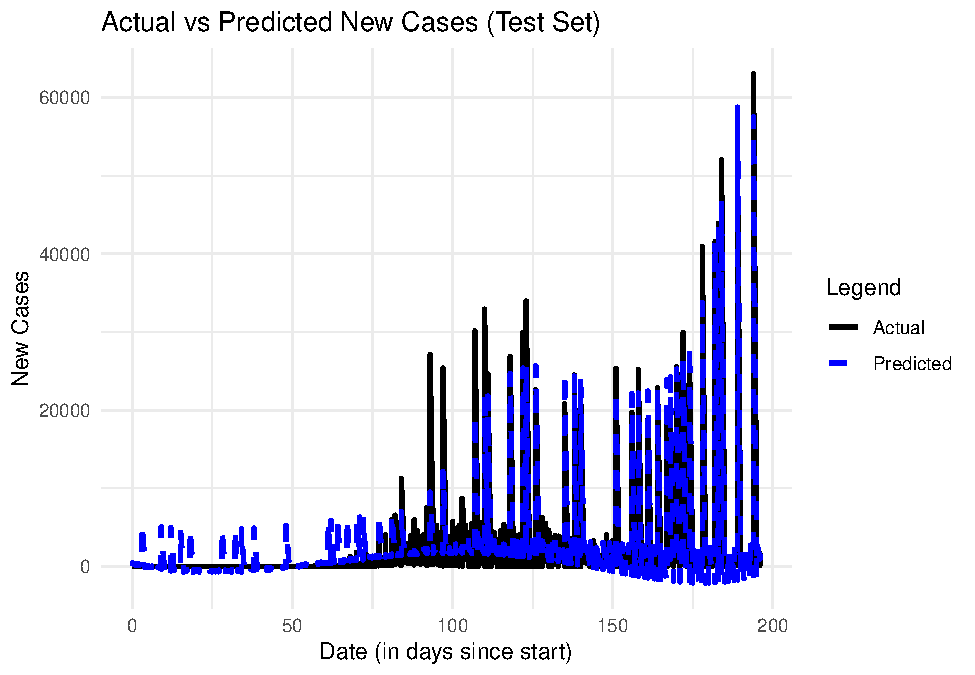
\includegraphics{Part_A_Covid_files/figure-latex/predict-new-cases-1.pdf}

\begin{Shaded}
\begin{Highlighting}[]
\CommentTok{\# Get the last 7 unique days in date\_num}
\NormalTok{last\_days }\OtherTok{\textless{}{-}} \FunctionTok{sort}\NormalTok{(}\FunctionTok{unique}\NormalTok{(test\_combined}\SpecialCharTok{$}\NormalTok{date\_num), }\AttributeTok{decreasing =} \ConstantTok{TRUE}\NormalTok{)[}\DecValTok{1}\SpecialCharTok{:}\DecValTok{7}\NormalTok{]}

\CommentTok{\# Filter test\_combined for only those days}
\NormalTok{last\_week\_predictions }\OtherTok{\textless{}{-}}\NormalTok{ test\_combined }\SpecialCharTok{\%\textgreater{}\%}
  \FunctionTok{filter}\NormalTok{(date\_num }\SpecialCharTok{\%in\%}\NormalTok{ last\_days) }\SpecialCharTok{\%\textgreater{}\%}
  \FunctionTok{arrange}\NormalTok{(date\_num, location)}

\CommentTok{\# Rename columns for clarity}
\NormalTok{last\_week\_predictions }\OtherTok{\textless{}{-}}\NormalTok{ last\_week\_predictions }\SpecialCharTok{\%\textgreater{}\%}
  \FunctionTok{select}\NormalTok{(date\_num, location, new\_cases, predicted\_new\_cases) }\SpecialCharTok{\%\textgreater{}\%}
  \FunctionTok{rename}\NormalTok{(}
    \AttributeTok{Days\_Since\_Start\_Date =}\NormalTok{ date\_num,}
    \AttributeTok{Location =}\NormalTok{ location,}
    \AttributeTok{Actual =}\NormalTok{ new\_cases,}
    \AttributeTok{Predicted =}\NormalTok{ predicted\_new\_cases}
\NormalTok{  )}

\CommentTok{\# Print the results}
\FunctionTok{print}\NormalTok{(last\_week\_predictions)}
\end{Highlighting}
\end{Shaded}

\begin{verbatim}
##    Days_Since_Start_Date       Location Actual  Predicted
## 1                    190      Australia    169 -1622.9947
## 2                    190      Australia    169 -1622.9947
## 3                    190      Australia    169 -1622.9947
## 4                    190      Australia    169 -1622.9947
## 5                    190         France    475   190.0016
## 6                    190         France    475   190.0016
## 7                    190         France    475   190.0016
## 8                    190         France    475   190.0016
## 9                    190 United Kingdom    581  2360.9782
## 10                   190 United Kingdom    581  2360.9782
## 11                   190 United Kingdom    581  2360.9782
## 12                   191      Australia    131 -1526.3437
## 13                   191      Australia    131 -1526.3437
## 14                   191         France    663   296.8814
## 15                   191         France    663   296.8814
## 16                   191         France    663   296.8814
## 17                   191         France    663   296.8814
## 18                   191         France    663   296.8814
## 19                   191          Italy    193  1317.9329
## 20                   191          Spain    543  1499.6738
## 21                   192      Australia    173 -1419.5294
## 22                   192      Australia    173 -1419.5294
## 23                   192      Australia    173 -1419.5294
## 24                   192         France    621   413.1488
## 25                   192 United Kingdom    642  2591.1252
## 26                   193      Australia    300 -1301.9346
## 27                   193      Australia    300 -1301.9346
## 28                   193      Australia    300 -1301.9346
## 29                   193      Australia    300 -1301.9346
## 30                   193         France    658   540.4300
## 31                   193         France    658   540.4300
## 32                   193          Italy    276  1550.6779
## 33                   193          Spain      0  1740.0381
## 34                   193 United Kingdom    512  2718.9370
## 35                   193 United Kingdom    512  2718.9370
## 36                   194      Australia    194 -1173.8962
## 37                   194      Australia    194 -1173.8962
## 38                   194      Australia    194 -1173.8962
## 39                   194      Australia    194 -1173.8962
## 40                   194         France      0   667.8793
## 41                   194         France      0   667.8793
## 42                   194 United Kingdom    820  2864.2155
## 43                   194 United Kingdom    820  2864.2155
## 44                   194  United States  63051 57534.9084
## 45                   195      Australia    244 -1034.5718
## 46                   195      Australia    244 -1034.5718
## 47                   195      Australia    244 -1034.5718
## 48                   195 United Kingdom    650  3016.9430
## 49                   195 United Kingdom    650  3016.9430
## 50                   195 United Kingdom    650  3016.9430
## 51                   195 United Kingdom    650  3016.9430
## 52                   196         France   1625   982.8076
## 53                   196         France   1625   982.8076
## 54                   196         France   1625   982.8076
## 55                   196         France   1625   982.8076
## 56                   196         France   1625   982.8076
## 57                   196         France   1625   982.8076
## 58                   196          Italy    169  1978.5706
## 59                   196 United Kingdom    530  3178.5747
## 60                   196 United Kingdom    530  3178.5747
\end{verbatim}

\vspace{1cm}

To show how the model performs, I will calculate the Root Mean Squared
Error (RMSE) and R-squared values for the predictions.

\begin{Shaded}
\begin{Highlighting}[]
\CommentTok{\# Calculate RMSE and R{-}squared}
\NormalTok{rmse }\OtherTok{\textless{}{-}} \FunctionTok{sqrt}\NormalTok{(}\FunctionTok{mean}\NormalTok{((test\_combined}\SpecialCharTok{$}\NormalTok{predicted\_new\_cases }\SpecialCharTok{{-}}\NormalTok{ test\_combined}\SpecialCharTok{$}\NormalTok{new\_cases)}\SpecialCharTok{\^{}}\DecValTok{2}\NormalTok{))}
\NormalTok{r\_squared }\OtherTok{\textless{}{-}} \DecValTok{1} \SpecialCharTok{{-}}\NormalTok{ (}\FunctionTok{sum}\NormalTok{((test\_combined}\SpecialCharTok{$}\NormalTok{predicted\_new\_cases }\SpecialCharTok{{-}}\NormalTok{ test\_combined}\SpecialCharTok{$}\NormalTok{new\_cases)}\SpecialCharTok{\^{}}\DecValTok{2}\NormalTok{) }\SpecialCharTok{/} \FunctionTok{sum}\NormalTok{((test\_combined}\SpecialCharTok{$}\NormalTok{new\_cases }\SpecialCharTok{{-}} \FunctionTok{mean}\NormalTok{(test\_combined}\SpecialCharTok{$}\NormalTok{new\_cases))}\SpecialCharTok{\^{}}\DecValTok{2}\NormalTok{))}
\FunctionTok{cat}\NormalTok{(}\StringTok{"RMSE: "}\NormalTok{, rmse, }\StringTok{"}\SpecialCharTok{\textbackslash{}n}\StringTok{"}\NormalTok{)}
\FunctionTok{cat}\NormalTok{(}\StringTok{"R{-}squared: "}\NormalTok{, r\_squared, }\StringTok{"}\SpecialCharTok{\textbackslash{}n}\StringTok{"}\NormalTok{)}
\end{Highlighting}
\end{Shaded}

\begin{verbatim}
## RMSE:  1599.545
\end{verbatim}

\begin{verbatim}
## R-squared:  0.866855
\end{verbatim}

\vspace{1cm}

To furthe validate the model, I will apply K-fold Cross-Validation to
evaluate the predictions.

\begin{Shaded}
\begin{Highlighting}[]
\FunctionTok{set.seed}\NormalTok{(}\DecValTok{4}\NormalTok{)}

\CommentTok{\# Create a control object for K{-}fold cross{-}validation}
\NormalTok{train\_control }\OtherTok{\textless{}{-}} \FunctionTok{trainControl}\NormalTok{(}\AttributeTok{method =} \StringTok{"cv"}\NormalTok{, }\AttributeTok{number =} \DecValTok{5}\NormalTok{)}

\CommentTok{\# Fit the model using K{-}fold cross{-}validation}
\NormalTok{cv\_model }\OtherTok{\textless{}{-}} \FunctionTok{train}\NormalTok{(}
\NormalTok{  new\_cases }\SpecialCharTok{\textasciitilde{}} \FunctionTok{poly}\NormalTok{(date\_num, }\DecValTok{5}\NormalTok{) }\SpecialCharTok{+} \FunctionTok{poly}\NormalTok{(total\_cases, }\DecValTok{6}\NormalTok{) }\SpecialCharTok{+}\NormalTok{ location,}
  \AttributeTok{data =}\NormalTok{ data\_higher\_gdp,}
  \AttributeTok{method =} \StringTok{"lm"}\NormalTok{,}
  \AttributeTok{trControl =}\NormalTok{ train\_control}
\NormalTok{)}

\CommentTok{\# Print the results of the cross{-}validation}
\FunctionTok{print}\NormalTok{(cv\_model)}
\end{Highlighting}
\end{Shaded}

\begin{verbatim}
## Linear Regression 
## 
## 5332 samples
##    3 predictor
## 
## No pre-processing
## Resampling: Cross-Validated (5 fold) 
## Summary of sample sizes: 4266, 4264, 4266, 4266, 4266 
## Resampling results:
## 
##   RMSE      Rsquared   MAE    
##   1782.621  0.8297452  1065.72
## 
## Tuning parameter 'intercept' was held constant at a value of TRUE
\end{verbatim}

Before applying K-fold Cross Validation, the model achieved an R-squared
of 0.87 and an RMSE of 1599.55, indicating a strong fit to the testing
data with realtively lower prediction error. However, after evaluating
the model using K-fold Cross Validation, the R-squared decreased
slightly to 0.83 and RMSE increased to 1782.62, indicating that the
model may be overfitting as it performs well on testing data but
struggles to generalise. The presence of outliers in the dataset may
have contributed to this discrepancy, as they can disproportionately
affect the model's performance, leading to higher RMSE and lower
R-squared values during cross-validation. Applying K-fold Cross
Validation helps to mitigate this issue by providing a more robust
evaluation of the model's performance across different subsets of the
data. However, in this instance, the model's performance on unseen data
is not as strong as it was on the testing data.

To further enhance the model's performance and generalisation
capabilities, steps such as outlier handling and feature selection may
be necessary. Although the sudden spikes in COVID-19 new cases might
appear as outliers from a statistical perspective, they could present
legitimate events such as outbreaks or changes in reporting practices.
Therefore, while outright removal of these points may not be
appropriate, techniques like robust regression or transformations could
be used to reducte the impact without disregarding meaningful data.
Moreover, applying feature selection helps lessen the noise from
irrelevant or redundant features, allowing the model to focus on the
most significant predictors. In this context, simply adding more data
may not yield better performance especially if the underlying patterns
remain volatile. Thus, refining the quality of the input data and
ensuring the model does not overly rely on extreme values are more
practical approaches to improve the model's predictive capabilities.
\vspace{1cm} \newpage

\section*{References}\label{references}
\addcontentsline{toc}{section}{References}

\phantomsection\label{refs}
\begin{CSLReferences}{1}{0}
\bibitem[\citeproctext]{ref-covidUSA}
Bergquist, S., Otten, T., \& Sarich, N. (2020). COVID-19 pandemic in the
united states. \emph{Health Policy and Technology}, \emph{9}(4),
623--638. \url{https://doi.org/10.1016/j.hlpt.2020.08.007}

\bibitem[\citeproctext]{ref-gdp}
Callen, T. (2025). \emph{Gross domestic product: An economy's all}.
\url{https://www.imf.org/en/Publications/fandd/issues/Series/Back-to-Basics/gross-domestic-product-GDP}

\bibitem[\citeproctext]{ref-covidtimeline}
Centers for Disease Control and Prevention. (2024). \emph{CDC museum
COVID-19 timeline}.
\url{https://www.cdc.gov/museum/timeline/covid19.html}

\bibitem[\citeproctext]{ref-covidEU}
Chadwick, L. (2020). \emph{How COVID-19 upended life in europe
throughout 2020}.
\url{https://www.euronews.com/2020/12/31/how-covid-19-upended-life-in-europe-throughout-2020}

\bibitem[\citeproctext]{ref-burunditourism}
Knoema Data Appliance. (2025). \emph{Burundi - leisure travel and
tourism spending in current prices}.
\url{https://opendataforafrica.org/atlas/Burundi/topics/Tourism/Leisure-Travel-and-Tourism-Spending/Leisure-travel-and-tourism-spending}

\bibitem[\citeproctext]{ref-luxembourgtourism}
macrotrends. (2025). \emph{Luxembourg tourism statistics 2002-2025}.
\url{https://www.macrotrends.net/global-metrics/countries/lux/luxembourg/tourism-statistics}

\bibitem[\citeproctext]{ref-covidmortality}
Tejada-Vera, B., S., M., \& Kramarow, E. A. (2022). \emph{COVID-19
mortality in adults aged 65 and over: United states, 2020}.
\url{https://www.cdc.gov/nchs/products/databriefs/db446.htm}

\bibitem[\citeproctext]{ref-worldgdp}
The World Factbook. (2025). \emph{Real GDP per capita}.
\url{http://cia.gov/the-world-factbook/field/real-gdp-per-capita/country-comparison/}

\end{CSLReferences}

\end{document}
